\documentclass[twoside]{book}

% Packages required by doxygen
\usepackage{fixltx2e}
\usepackage{calc}
\usepackage{doxygen}
\usepackage{graphicx}
\usepackage[utf8]{inputenc}
\usepackage{makeidx}
\usepackage{multicol}
\usepackage{multirow}
\PassOptionsToPackage{warn}{textcomp}
\usepackage{textcomp}
\usepackage[nointegrals]{wasysym}
\usepackage[table]{xcolor}

% Font selection
\usepackage[T1]{fontenc}
\usepackage{mathptmx}
\usepackage[scaled=.90]{helvet}
\usepackage{courier}
\usepackage{amssymb}
\usepackage{sectsty}
\renewcommand{\familydefault}{\sfdefault}
\allsectionsfont{%
  \fontseries{bc}\selectfont%
  \color{darkgray}%
}
\renewcommand{\DoxyLabelFont}{%
  \fontseries{bc}\selectfont%
  \color{darkgray}%
}
\newcommand{\+}{\discretionary{\mbox{\scriptsize$\hookleftarrow$}}{}{}}

% Page & text layout
\usepackage{geometry}
\geometry{%
  a4paper,%
  top=2.5cm,%
  bottom=2.5cm,%
  left=2.5cm,%
  right=2.5cm%
}
\tolerance=750
\hfuzz=15pt
\hbadness=750
\setlength{\emergencystretch}{15pt}
\setlength{\parindent}{0cm}
\setlength{\parskip}{0.2cm}
\makeatletter
\renewcommand{\paragraph}{%
  \@startsection{paragraph}{4}{0ex}{-1.0ex}{1.0ex}{%
    \normalfont\normalsize\bfseries\SS@parafont%
  }%
}
\renewcommand{\subparagraph}{%
  \@startsection{subparagraph}{5}{0ex}{-1.0ex}{1.0ex}{%
    \normalfont\normalsize\bfseries\SS@subparafont%
  }%
}
\makeatother

% Headers & footers
\usepackage{fancyhdr}
\pagestyle{fancyplain}
\fancyhead[LE]{\fancyplain{}{\bfseries\thepage}}
\fancyhead[CE]{\fancyplain{}{}}
\fancyhead[RE]{\fancyplain{}{\bfseries\leftmark}}
\fancyhead[LO]{\fancyplain{}{\bfseries\rightmark}}
\fancyhead[CO]{\fancyplain{}{}}
\fancyhead[RO]{\fancyplain{}{\bfseries\thepage}}
\fancyfoot[LE]{\fancyplain{}{}}
\fancyfoot[CE]{\fancyplain{}{}}
\fancyfoot[RE]{\fancyplain{}{\bfseries\scriptsize Generated on Fri Feb 24 2017 12\+:24\+:06 for Lab2\+: Estructuras de Datos Lineales by Doxygen }}
\fancyfoot[LO]{\fancyplain{}{\bfseries\scriptsize Generated on Fri Feb 24 2017 12\+:24\+:06 for Lab2\+: Estructuras de Datos Lineales by Doxygen }}
\fancyfoot[CO]{\fancyplain{}{}}
\fancyfoot[RO]{\fancyplain{}{}}
\renewcommand{\footrulewidth}{0.4pt}
\renewcommand{\chaptermark}[1]{%
  \markboth{#1}{}%
}
\renewcommand{\sectionmark}[1]{%
  \markright{\thesection\ #1}%
}

% Indices & bibliography
\usepackage{natbib}
\usepackage[titles]{tocloft}
\setcounter{tocdepth}{3}
\setcounter{secnumdepth}{5}
\makeindex

% Hyperlinks (required, but should be loaded last)
\usepackage{ifpdf}
\ifpdf
  \usepackage[pdftex,pagebackref=true]{hyperref}
\else
  \usepackage[ps2pdf,pagebackref=true]{hyperref}
\fi
\hypersetup{%
  colorlinks=true,%
  linkcolor=blue,%
  citecolor=blue,%
  unicode%
}

% Custom commands
\newcommand{\clearemptydoublepage}{%
  \newpage{\pagestyle{empty}\cleardoublepage}%
}


%===== C O N T E N T S =====

\begin{document}

% Titlepage & ToC
\hypersetup{pageanchor=false,
             bookmarks=true,
             bookmarksnumbered=true,
             pdfencoding=unicode
            }
\pagenumbering{roman}
\begin{titlepage}
\vspace*{7cm}
\begin{center}%
{\Large Lab2\+: Estructuras de Datos Lineales \\[1ex]\large v1.\+0 }\\
\vspace*{1cm}
{\large Generated by Doxygen 1.8.8}\\
\vspace*{0.5cm}
{\small Fri Feb 24 2017 12:24:06}\\
\end{center}
\end{titlepage}
\clearemptydoublepage
\tableofcontents
\clearemptydoublepage
\pagenumbering{arabic}
\hypersetup{pageanchor=true}

%--- Begin generated contents ---
\chapter{Hierarchical Index}
\section{Class Hierarchy}
This inheritance list is sorted roughly, but not completely, alphabetically\+:\begin{DoxyCompactList}
\item \contentsline{section}{B\+S\+T$<$ Data $>$}{\pageref{class_b_s_t}}{}
\item \contentsline{section}{Cell$<$ D $>$}{\pageref{class_cell}}{}
\item \contentsline{section}{Cell$<$ Edge$<$ Data $>$ $>$}{\pageref{class_cell}}{}
\item \contentsline{section}{Cell$<$ Node$<$ D $>$ $>$}{\pageref{class_cell}}{}
\item \contentsline{section}{Cell$<$ Node$<$ Data $>$ $>$}{\pageref{class_cell}}{}
\item \contentsline{section}{Data$<$ D $>$}{\pageref{class_data}}{}
\item \contentsline{section}{Edge$<$ D $>$}{\pageref{class_edge}}{}
\item \contentsline{section}{Edge$<$ Data $>$}{\pageref{class_edge}}{}
\item \contentsline{section}{Graph$<$ Data $>$}{\pageref{class_graph}}{}
\item \contentsline{section}{Graph\+With\+Array}{\pageref{class_graph_with_array}}{}
\item \contentsline{section}{List$<$ D, P $>$}{\pageref{class_list}}{}
\begin{DoxyCompactList}
\item \contentsline{section}{List\+With\+Array$<$ D, P $>$}{\pageref{class_list_with_array}}{}
\item \contentsline{section}{List\+With\+Pointer$<$ D, P $>$}{\pageref{class_list_with_pointer}}{}
\end{DoxyCompactList}
\item \contentsline{section}{List$<$ Edge$<$ Data $>$, Cell$<$ Edge$<$ Data $>$ $>$ $\ast$ $>$}{\pageref{class_list}}{}
\begin{DoxyCompactList}
\item \contentsline{section}{List\+With\+Pointer$<$ Edge$<$ Data $>$, Cell$<$ Edge$<$ Data $>$ $>$ $\ast$ $>$}{\pageref{class_list_with_pointer}}{}
\end{DoxyCompactList}
\item \contentsline{section}{List$<$ N\+O\+D\+E, int $>$}{\pageref{class_list}}{}
\item \contentsline{section}{List$<$ Node$<$ D $>$, Cell$<$ Node$<$ D $>$ $>$ $\ast$ $>$}{\pageref{class_list}}{}
\begin{DoxyCompactList}
\item \contentsline{section}{List\+With\+Pointer$<$ Node$<$ D $>$, Cell$<$ Node$<$ D $>$ $>$ $\ast$ $>$}{\pageref{class_list_with_pointer}}{}
\end{DoxyCompactList}
\item \contentsline{section}{List$<$ Node$<$ Data $>$, Cell$<$ Node$<$ Data $>$ $>$ $\ast$ $>$}{\pageref{class_list}}{}
\begin{DoxyCompactList}
\item \contentsline{section}{List\+With\+Pointer$<$ Node$<$ Data $>$, Cell$<$ Node$<$ Data $>$ $>$ $\ast$ $>$}{\pageref{class_list_with_pointer}}{}
\end{DoxyCompactList}
\item \contentsline{section}{My\+Data$<$ D $>$}{\pageref{class_my_data}}{}
\item \contentsline{section}{Node$<$ D $>$}{\pageref{class_node}}{}
\item \contentsline{section}{Node$<$ Data $>$}{\pageref{class_node}}{}
\end{DoxyCompactList}

\chapter{Class Index}
\section{Class List}
Here are the classes, structs, unions and interfaces with brief descriptions\+:\begin{DoxyCompactList}
\item\contentsline{section}{\hyperlink{class_d_n_acompare}{D\+N\+Acompare} }{\pageref{class_d_n_acompare}}{}
\item\contentsline{section}{\hyperlink{class_graph_aho_corasick}{Graph\+Aho\+Corasick} }{\pageref{class_graph_aho_corasick}}{}
\item\contentsline{section}{\hyperlink{class_list}{List$<$ D, P $>$} \\*Libreria que genera un template de una clase abstracta list }{\pageref{class_list}}{}
\item\contentsline{section}{\hyperlink{class_list_with_array}{List\+With\+Array$<$ D, P $>$} \\*Libreria que genera un template de una clase \hyperlink{class_list_with_array}{List\+With\+Array} (lista implementada con arreglos) que hereda de la clase \hyperlink{class_list}{List} y que toma un tipo de dato para los datos contenidos en la lista (D) y otro para los indices de las misma (P) }{\pageref{class_list_with_array}}{}
\item\contentsline{section}{\hyperlink{class_stade}{Stade} }{\pageref{class_stade}}{}
\item\contentsline{section}{\hyperlink{class_stade_suc}{Stade\+Suc} }{\pageref{class_stade_suc}}{}
\end{DoxyCompactList}

\chapter{File Index}
\section{File List}
Here is a list of all files with brief descriptions\+:\begin{DoxyCompactList}
\item\contentsline{section}{include/\hyperlink{_cell_8h}{Cell.\+h} }{\pageref{_cell_8h}}{}
\item\contentsline{section}{include/\hyperlink{_list_8h}{List.\+h} }{\pageref{_list_8h}}{}
\item\contentsline{section}{include/\hyperlink{_list_with_array_8h}{List\+With\+Array.\+h} }{\pageref{_list_with_array_8h}}{}
\item\contentsline{section}{include/\hyperlink{_list_with_pointer_8h}{List\+With\+Pointer.\+h} }{\pageref{_list_with_pointer_8h}}{}
\item\contentsline{section}{include/\hyperlink{_queue_8h}{Queue.\+h} }{\pageref{_queue_8h}}{}
\item\contentsline{section}{include/\hyperlink{_stack_8h}{Stack.\+h} }{\pageref{_stack_8h}}{}
\item\contentsline{section}{src/\hyperlink{main_8cpp}{main.\+cpp} }{\pageref{main_8cpp}}{}
\end{DoxyCompactList}

\chapter{Class Documentation}
\hypertarget{class_cell}{\section{Cell$<$ D $>$ Class Template Reference}
\label{class_cell}\index{Cell$<$ D $>$@{Cell$<$ D $>$}}
}


Libreria que genera un template de una clase \hyperlink{class_cell}{Cell} que contiene datos de tipo D.  




{\ttfamily \#include $<$Cell.\+h$>$}



Collaboration diagram for Cell$<$ D $>$\+:
\subsection*{Public Member Functions}
\begin{DoxyCompactItemize}
\item 
\hyperlink{class_cell_a742a2adf7fa420fa9cbe386a87b5c79b}{Cell} ()
\begin{DoxyCompactList}\small\item\em Constructor de la clase \hyperlink{class_cell}{Cell}. \end{DoxyCompactList}\item 
\hyperlink{class_cell_addb102d2635522a2858eef6687407bcb}{Cell} (\hyperlink{gwp_2main_8cpp_af316c33cc298530f245e8b55330e86b5}{D} $\ast$d, \hyperlink{class_cell}{Cell} $\ast$n)
\begin{DoxyCompactList}\small\item\em Constructor sobrecargado de la clase \hyperlink{class_cell}{Cell}. \end{DoxyCompactList}\item 
\hyperlink{class_cell_a545129618ba41b218c6be7293975efda}{$\sim$\+Cell} ()
\begin{DoxyCompactList}\small\item\em Destructor de la clase \hyperlink{class_cell}{Cell}. \end{DoxyCompactList}\end{DoxyCompactItemize}
\subsection*{Public Attributes}
\begin{DoxyCompactItemize}
\item 
\hyperlink{class_cell}{Cell} $\ast$ \hyperlink{class_cell_a7e0e6c090f8aca70862c2dbc3257e3b9}{next}
\begin{DoxyCompactList}\small\item\em Atrib. \end{DoxyCompactList}\item 
\hyperlink{gwp_2main_8cpp_af316c33cc298530f245e8b55330e86b5}{D} $\ast$ \hyperlink{class_cell_ab8cc4d3059ef84a652eabc05b6c28f49}{data}
\begin{DoxyCompactList}\small\item\em Atrib. \end{DoxyCompactList}\end{DoxyCompactItemize}


\subsection{Detailed Description}
\subsubsection*{template$<$typename D$>$class Cell$<$ D $>$}

Libreria que genera un template de una clase \hyperlink{class_cell}{Cell} que contiene datos de tipo D. 

Definition at line 17 of file Cell.\+h.



\subsection{Constructor \& Destructor Documentation}
\hypertarget{class_cell_a742a2adf7fa420fa9cbe386a87b5c79b}{\index{Cell@{Cell}!Cell@{Cell}}
\index{Cell@{Cell}!Cell@{Cell}}
\subsubsection[{Cell}]{\setlength{\rightskip}{0pt plus 5cm}template$<$typename D$>$ {\bf Cell}$<$ {\bf D} $>$\+::{\bf Cell} (
\begin{DoxyParamCaption}
{}
\end{DoxyParamCaption}
)\hspace{0.3cm}{\ttfamily [inline]}}}\label{class_cell_a742a2adf7fa420fa9cbe386a87b5c79b}


Constructor de la clase \hyperlink{class_cell}{Cell}. 



Definition at line 25 of file Cell.\+h.

\hypertarget{class_cell_addb102d2635522a2858eef6687407bcb}{\index{Cell@{Cell}!Cell@{Cell}}
\index{Cell@{Cell}!Cell@{Cell}}
\subsubsection[{Cell}]{\setlength{\rightskip}{0pt plus 5cm}template$<$typename D$>$ {\bf Cell}$<$ {\bf D} $>$\+::{\bf Cell} (
\begin{DoxyParamCaption}
\item[{{\bf D} $\ast$}]{d, }
\item[{{\bf Cell}$<$ {\bf D} $>$ $\ast$}]{n}
\end{DoxyParamCaption}
)\hspace{0.3cm}{\ttfamily [inline]}}}\label{class_cell_addb102d2635522a2858eef6687407bcb}


Constructor sobrecargado de la clase \hyperlink{class_cell}{Cell}. 


\begin{DoxyParams}{Parameters}
{\em d} & Puntero al dato de tipo D que se asigna a la celda \\
\hline
{\em n} & Puntero a la celda siguiente de la celda que se crea \\
\hline
\end{DoxyParams}


Definition at line 35 of file Cell.\+h.

\hypertarget{class_cell_a545129618ba41b218c6be7293975efda}{\index{Cell@{Cell}!````~Cell@{$\sim$\+Cell}}
\index{````~Cell@{$\sim$\+Cell}!Cell@{Cell}}
\subsubsection[{$\sim$\+Cell}]{\setlength{\rightskip}{0pt plus 5cm}template$<$typename D$>$ {\bf Cell}$<$ {\bf D} $>$\+::$\sim${\bf Cell} (
\begin{DoxyParamCaption}
{}
\end{DoxyParamCaption}
)\hspace{0.3cm}{\ttfamily [inline]}}}\label{class_cell_a545129618ba41b218c6be7293975efda}


Destructor de la clase \hyperlink{class_cell}{Cell}. 



Definition at line 43 of file Cell.\+h.



\subsection{Member Data Documentation}
\hypertarget{class_cell_ab8cc4d3059ef84a652eabc05b6c28f49}{\index{Cell@{Cell}!data@{data}}
\index{data@{data}!Cell@{Cell}}
\subsubsection[{data}]{\setlength{\rightskip}{0pt plus 5cm}template$<$typename D$>$ {\bf D}$\ast$ {\bf Cell}$<$ {\bf D} $>$\+::data}}\label{class_cell_ab8cc4d3059ef84a652eabc05b6c28f49}


Atrib. 

publico de tipo puntero a D que indica el dato incluido en la celda 

Definition at line 20 of file Cell.\+h.

\hypertarget{class_cell_a7e0e6c090f8aca70862c2dbc3257e3b9}{\index{Cell@{Cell}!next@{next}}
\index{next@{next}!Cell@{Cell}}
\subsubsection[{next}]{\setlength{\rightskip}{0pt plus 5cm}template$<$typename D$>$ {\bf Cell}$\ast$ {\bf Cell}$<$ {\bf D} $>$\+::next}}\label{class_cell_a7e0e6c090f8aca70862c2dbc3257e3b9}


Atrib. 

publico de tipo puntero a \hyperlink{class_cell}{Cell} que indica la siguiente celda 

Definition at line 19 of file Cell.\+h.



The documentation for this class was generated from the following file\+:\begin{DoxyCompactItemize}
\item 
include/gwp/\hyperlink{_cell_8h}{Cell.\+h}\end{DoxyCompactItemize}

\hypertarget{class_list}{\section{List$<$ D, P $>$ Class Template Reference}
\label{class_list}\index{List$<$ D, P $>$@{List$<$ D, P $>$}}
}


Libreria que genera un template de una clase abstracta list.  




{\ttfamily \#include $<$List.\+h$>$}

Inheritance diagram for List$<$ D, P $>$\+:\begin{figure}[H]
\begin{center}
\leavevmode
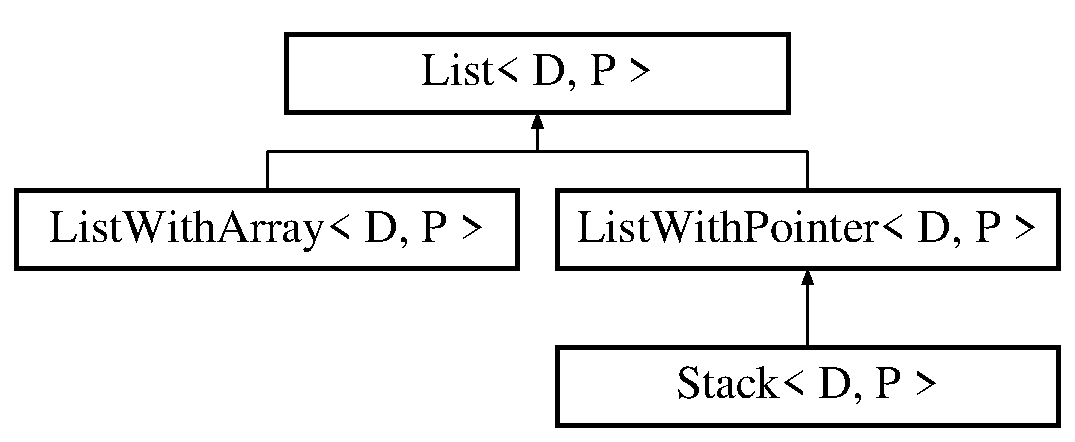
\includegraphics[height=3.000000cm]{class_list}
\end{center}
\end{figure}
\subsection*{Public Member Functions}
\begin{DoxyCompactItemize}
\item 
\hyperlink{class_list_a3deb54ab4f51c6c39aa4015f258b5812}{List} ()
\begin{DoxyCompactList}\small\item\em Constructor de la clase \hyperlink{class_list}{List}. \end{DoxyCompactList}\item 
virtual \hyperlink{class_list_a624593fb77847bf7ad4cacfba3442471}{$\sim$\+List} ()
\begin{DoxyCompactList}\small\item\em Destructor de la clase \hyperlink{class_list}{List}. \end{DoxyCompactList}\item 
virtual void \hyperlink{class_list_a01f588d87d47f8332928eca38f7b11bb}{insert} (D d)=0
\begin{DoxyCompactList}\small\item\em Metodo virtual puro para insercion de datos en \hyperlink{class_list}{List}. \end{DoxyCompactList}\item 
virtual void \hyperlink{class_list_a14fc4e853102018df78db3899aa00d71}{remove} (D d)=0
\begin{DoxyCompactList}\small\item\em Metodo virtual puro para la remocion de un dato especifico de \hyperlink{class_list}{List}. \end{DoxyCompactList}\item 
virtual P \hyperlink{class_list_a2b40d6fffc7b2fb5138b648f52c839ee}{find} (D d)=0
\begin{DoxyCompactList}\small\item\em Metodo virtual puro para la busqueda de un dato especifico en \hyperlink{class_list}{List}. \end{DoxyCompactList}\item 
virtual D \hyperlink{class_list_a5bd565e668247ae0691983227367cc88}{get} (P k)=0
\begin{DoxyCompactList}\small\item\em Metodo virtual puro para obtener un dato en \hyperlink{class_list}{List}. \end{DoxyCompactList}\item 
virtual void \hyperlink{class_list_acb062aa988f4048498b30a2d845a311b}{assign} (P k, D d)=0
\begin{DoxyCompactList}\small\item\em Metodo virtual puro para asignar un valor especifico a un dato en \hyperlink{class_list}{List}. \end{DoxyCompactList}\item 
virtual void \hyperlink{class_list_ae3795939f27cf3e688cd470450e0c27a}{sort} ()=0
\begin{DoxyCompactList}\small\item\em Metodo virtual puro para ordenar \hyperlink{class_list}{List}. \end{DoxyCompactList}\item 
virtual int \hyperlink{class_list_af213bbcf13ee436a0f04cde66e337672}{get\+Size} ()=0
\begin{DoxyCompactList}\small\item\em Metodo virtual puro para obtener el tamaño de \hyperlink{class_list}{List}. \end{DoxyCompactList}\item 
virtual void \hyperlink{class_list_a8b34931e187e7e6b86aad86510ce4f3b}{print\+List} ()=0
\begin{DoxyCompactList}\small\item\em Metodo virtual puro para imrprimir \hyperlink{class_list}{List}. \end{DoxyCompactList}\item 
virtual P \hyperlink{class_list_a4ec3e88e176bb45bc49b030d1c8abb3f}{next} (P k)=0
\begin{DoxyCompactList}\small\item\em Metodo virtual puro para obtener el siguiente elemento de una posicion especifica de \hyperlink{class_list}{List}. \end{DoxyCompactList}\item 
virtual P \hyperlink{class_list_acc1831ae92a288345ef20cb29f3846b2}{prev} (P k)=0
\begin{DoxyCompactList}\small\item\em Metodo virtual puro para obtener el elemento anterior de una posicion especifica de \hyperlink{class_list}{List}. \end{DoxyCompactList}\item 
virtual void \hyperlink{class_list_a24b4f177a70215980e81ef7b2981fa1e}{empty\+List} ()=0
\begin{DoxyCompactList}\small\item\em Metodo virtual puro para vaciar \hyperlink{class_list}{List}\+: Deja sin ningun elemento \hyperlink{class_list}{List}. \end{DoxyCompactList}\end{DoxyCompactItemize}
\subsection*{Protected Attributes}
\begin{DoxyCompactItemize}
\item 
int \hyperlink{class_list_aa61221b9bda8b2b56a61bd869daacbfd}{n}
\begin{DoxyCompactList}\small\item\em Atrib. \end{DoxyCompactList}\item 
P \hyperlink{class_list_a32b9741aa48daca064edf0e83abf7a0f}{last}
\begin{DoxyCompactList}\small\item\em Atrib. \end{DoxyCompactList}\end{DoxyCompactItemize}


\subsection{Detailed Description}
\subsubsection*{template$<$typename D, typename P$>$class List$<$ D, P $>$}

Libreria que genera un template de una clase abstracta list. 

\begin{DoxyAuthor}{Author}
Luis Adrian Aguilar -\/ B00092 

Robin Gonzalez Ricz -\/ B43011 

Giancarlo Marin -\/ B54099 
\end{DoxyAuthor}
\begin{DoxyDate}{Date}
21-\/02-\/2017 Libreria que genera un template de una clase abstracta list que toma un tipo de dato para los datos contenidos en la lista (D) y otro para los indices de las misma (P) 
\end{DoxyDate}


\subsection{Constructor \& Destructor Documentation}
\hypertarget{class_list_a3deb54ab4f51c6c39aa4015f258b5812}{\index{List@{List}!List@{List}}
\index{List@{List}!List@{List}}
\subsubsection[{List}]{\setlength{\rightskip}{0pt plus 5cm}template$<$typename D , typename P $>$ {\bf List}$<$ D, P $>$\+::{\bf List} (
\begin{DoxyParamCaption}
{}
\end{DoxyParamCaption}
)\hspace{0.3cm}{\ttfamily [inline]}}}\label{class_list_a3deb54ab4f51c6c39aa4015f258b5812}


Constructor de la clase \hyperlink{class_list}{List}. 

\hypertarget{class_list_a624593fb77847bf7ad4cacfba3442471}{\index{List@{List}!````~List@{$\sim$\+List}}
\index{````~List@{$\sim$\+List}!List@{List}}
\subsubsection[{$\sim$\+List}]{\setlength{\rightskip}{0pt plus 5cm}template$<$typename D , typename P $>$ virtual {\bf List}$<$ D, P $>$\+::$\sim${\bf List} (
\begin{DoxyParamCaption}
{}
\end{DoxyParamCaption}
)\hspace{0.3cm}{\ttfamily [inline]}, {\ttfamily [virtual]}}}\label{class_list_a624593fb77847bf7ad4cacfba3442471}


Destructor de la clase \hyperlink{class_list}{List}. 



\subsection{Member Function Documentation}
\hypertarget{class_list_acb062aa988f4048498b30a2d845a311b}{\index{List@{List}!assign@{assign}}
\index{assign@{assign}!List@{List}}
\subsubsection[{assign}]{\setlength{\rightskip}{0pt plus 5cm}template$<$typename D , typename P $>$ virtual void {\bf List}$<$ D, P $>$\+::assign (
\begin{DoxyParamCaption}
\item[{P}]{k, }
\item[{D}]{d}
\end{DoxyParamCaption}
)\hspace{0.3cm}{\ttfamily [pure virtual]}}}\label{class_list_acb062aa988f4048498b30a2d845a311b}


Metodo virtual puro para asignar un valor especifico a un dato en \hyperlink{class_list}{List}. 


\begin{DoxyParams}{Parameters}
{\em k} & Indice de tipo P dentro de list donde se asignara el nuevo valor \\
\hline
{\em d} & Dato de tipo D que se asigna en la posicion k \\
\hline
\end{DoxyParams}


Implemented in \hyperlink{class_list_with_array_a9dd1fd2337c6c8d437de71aae0e816c8}{List\+With\+Array$<$ D, P $>$}, and \hyperlink{class_list_with_pointer_aeaa834b22c4d7276a77ff29df3da7a30}{List\+With\+Pointer$<$ D, P $>$}.

\hypertarget{class_list_a24b4f177a70215980e81ef7b2981fa1e}{\index{List@{List}!empty\+List@{empty\+List}}
\index{empty\+List@{empty\+List}!List@{List}}
\subsubsection[{empty\+List}]{\setlength{\rightskip}{0pt plus 5cm}template$<$typename D , typename P $>$ virtual void {\bf List}$<$ D, P $>$\+::empty\+List (
\begin{DoxyParamCaption}
{}
\end{DoxyParamCaption}
)\hspace{0.3cm}{\ttfamily [pure virtual]}}}\label{class_list_a24b4f177a70215980e81ef7b2981fa1e}


Metodo virtual puro para vaciar \hyperlink{class_list}{List}\+: Deja sin ningun elemento \hyperlink{class_list}{List}. 



Implemented in \hyperlink{class_list_with_pointer_aec4f5374971962c79d397bbcd0080199}{List\+With\+Pointer$<$ D, P $>$}, and \hyperlink{class_list_with_array_a2179e228f285cc29b46bd5d13ba0b4ed}{List\+With\+Array$<$ D, P $>$}.

\hypertarget{class_list_a2b40d6fffc7b2fb5138b648f52c839ee}{\index{List@{List}!find@{find}}
\index{find@{find}!List@{List}}
\subsubsection[{find}]{\setlength{\rightskip}{0pt plus 5cm}template$<$typename D , typename P $>$ virtual P {\bf List}$<$ D, P $>$\+::find (
\begin{DoxyParamCaption}
\item[{D}]{d}
\end{DoxyParamCaption}
)\hspace{0.3cm}{\ttfamily [pure virtual]}}}\label{class_list_a2b40d6fffc7b2fb5138b648f52c839ee}


Metodo virtual puro para la busqueda de un dato especifico en \hyperlink{class_list}{List}. 


\begin{DoxyParams}{Parameters}
{\em d} & Dato que se desea buscar en \hyperlink{class_list}{List} \\
\hline
\end{DoxyParams}
\begin{DoxyReturn}{Returns}
Indice de tipo P dentro de \hyperlink{class_list}{List} 
\end{DoxyReturn}


Implemented in \hyperlink{class_stack_aa8a3a0b773900e44f641e3be9d9345da}{Stack$<$ D, P $>$}, \hyperlink{class_list_with_array_a9a054a6d407dc5cb39575739fe412fff}{List\+With\+Array$<$ D, P $>$}, \hyperlink{class_queue_a5c5ad7000d15506d3ec9c2ef6c8e6041}{Queue$<$ D, P $>$}, and \hyperlink{class_list_with_pointer_afeff8b963c197378553e2a3f73eaf66a}{List\+With\+Pointer$<$ D, P $>$}.

\hypertarget{class_list_a5bd565e668247ae0691983227367cc88}{\index{List@{List}!get@{get}}
\index{get@{get}!List@{List}}
\subsubsection[{get}]{\setlength{\rightskip}{0pt plus 5cm}template$<$typename D , typename P $>$ virtual D {\bf List}$<$ D, P $>$\+::get (
\begin{DoxyParamCaption}
\item[{P}]{k}
\end{DoxyParamCaption}
)\hspace{0.3cm}{\ttfamily [pure virtual]}}}\label{class_list_a5bd565e668247ae0691983227367cc88}


Metodo virtual puro para obtener un dato en \hyperlink{class_list}{List}. 


\begin{DoxyParams}{Parameters}
{\em k} & Indice de tipo P dentro de \hyperlink{class_list}{List} del que se desea obtener dato \\
\hline
\end{DoxyParams}
\begin{DoxyReturn}{Returns}
Dato contenido en k de tipo D 
\end{DoxyReturn}


Implemented in \hyperlink{class_list_with_array_a20cfc82811967bc2a77a6e43b9cebb46}{List\+With\+Array$<$ D, P $>$}, and \hyperlink{class_list_with_pointer_a0ff36c852334da8bc167356e636c1846}{List\+With\+Pointer$<$ D, P $>$}.

\hypertarget{class_list_af213bbcf13ee436a0f04cde66e337672}{\index{List@{List}!get\+Size@{get\+Size}}
\index{get\+Size@{get\+Size}!List@{List}}
\subsubsection[{get\+Size}]{\setlength{\rightskip}{0pt plus 5cm}template$<$typename D , typename P $>$ virtual int {\bf List}$<$ D, P $>$\+::get\+Size (
\begin{DoxyParamCaption}
{}
\end{DoxyParamCaption}
)\hspace{0.3cm}{\ttfamily [pure virtual]}}}\label{class_list_af213bbcf13ee436a0f04cde66e337672}


Metodo virtual puro para obtener el tamaño de \hyperlink{class_list}{List}. 



Implemented in \hyperlink{class_list_with_pointer_ac70c49b5703887fd867e90cdac3c706f}{List\+With\+Pointer$<$ D, P $>$}, \hyperlink{class_list_with_array_ae7a071bcdde9ddbf4c40a716f5a09434}{List\+With\+Array$<$ D, P $>$}, \hyperlink{class_stack_a74fc7e5921dfb247f9ad7052c3c4297a}{Stack$<$ D, P $>$}, and \hyperlink{class_queue_ab2c7217e6737bf579493b321184a2db3}{Queue$<$ D, P $>$}.

\hypertarget{class_list_a01f588d87d47f8332928eca38f7b11bb}{\index{List@{List}!insert@{insert}}
\index{insert@{insert}!List@{List}}
\subsubsection[{insert}]{\setlength{\rightskip}{0pt plus 5cm}template$<$typename D , typename P $>$ virtual void {\bf List}$<$ D, P $>$\+::insert (
\begin{DoxyParamCaption}
\item[{D}]{d}
\end{DoxyParamCaption}
)\hspace{0.3cm}{\ttfamily [pure virtual]}}}\label{class_list_a01f588d87d47f8332928eca38f7b11bb}


Metodo virtual puro para insercion de datos en \hyperlink{class_list}{List}. 


\begin{DoxyParams}{Parameters}
{\em d} & Dato de tipo D que se desea insertar en \hyperlink{class_list}{List} \\
\hline
\end{DoxyParams}


Implemented in \hyperlink{class_list_with_array_afa0b6d215c2cc1d3fe6b9b48d6b6917d}{List\+With\+Array$<$ D, P $>$}, and \hyperlink{class_list_with_pointer_a676e57683ade8e179e8eff5885f7309a}{List\+With\+Pointer$<$ D, P $>$}.

\hypertarget{class_list_a4ec3e88e176bb45bc49b030d1c8abb3f}{\index{List@{List}!next@{next}}
\index{next@{next}!List@{List}}
\subsubsection[{next}]{\setlength{\rightskip}{0pt plus 5cm}template$<$typename D , typename P $>$ virtual P {\bf List}$<$ D, P $>$\+::next (
\begin{DoxyParamCaption}
\item[{P}]{k}
\end{DoxyParamCaption}
)\hspace{0.3cm}{\ttfamily [pure virtual]}}}\label{class_list_a4ec3e88e176bb45bc49b030d1c8abb3f}


Metodo virtual puro para obtener el siguiente elemento de una posicion especifica de \hyperlink{class_list}{List}. 


\begin{DoxyParams}{Parameters}
{\em k} & Indice de tipo P dentro de \hyperlink{class_list}{List} del que se desea el siguiente elemento \\
\hline
\end{DoxyParams}
\begin{DoxyReturn}{Returns}
Siguiente elemento de k de tipo P 
\end{DoxyReturn}


Implemented in \hyperlink{class_list_with_pointer_a518b5ee89e3ad32ae7cd4ddd5d4fa7e9}{List\+With\+Pointer$<$ D, P $>$}, \hyperlink{class_list_with_array_a125811011abb77c1b11e5150f4524fb1}{List\+With\+Array$<$ D, P $>$}, \hyperlink{class_queue_aa4c9b83f260a172e1fffc389f354386f}{Queue$<$ D, P $>$}, and \hyperlink{class_stack_ab7f8f7e4ab10c00769c1debc5391fc17}{Stack$<$ D, P $>$}.

\hypertarget{class_list_acc1831ae92a288345ef20cb29f3846b2}{\index{List@{List}!prev@{prev}}
\index{prev@{prev}!List@{List}}
\subsubsection[{prev}]{\setlength{\rightskip}{0pt plus 5cm}template$<$typename D , typename P $>$ virtual P {\bf List}$<$ D, P $>$\+::prev (
\begin{DoxyParamCaption}
\item[{P}]{k}
\end{DoxyParamCaption}
)\hspace{0.3cm}{\ttfamily [pure virtual]}}}\label{class_list_acc1831ae92a288345ef20cb29f3846b2}


Metodo virtual puro para obtener el elemento anterior de una posicion especifica de \hyperlink{class_list}{List}. 


\begin{DoxyParams}{Parameters}
{\em k} & Indice de tipo P dentro de \hyperlink{class_list}{List} del que se desea el elemento anterior \\
\hline
\end{DoxyParams}
\begin{DoxyReturn}{Returns}
Elemento anterior de k de tipo P 
\end{DoxyReturn}


Implemented in \hyperlink{class_list_with_pointer_a7242068fcc3a193f0f7e94517856e431}{List\+With\+Pointer$<$ D, P $>$}, \hyperlink{class_list_with_array_a72f0d74c4ae1fd4697088114db41d442}{List\+With\+Array$<$ D, P $>$}, \hyperlink{class_queue_adcb9a0e709ea65bc7e98f7e9cbae8a39}{Queue$<$ D, P $>$}, and \hyperlink{class_stack_a0c0b55f72c9249bfb9252bce1a93458d}{Stack$<$ D, P $>$}.

\hypertarget{class_list_a8b34931e187e7e6b86aad86510ce4f3b}{\index{List@{List}!print\+List@{print\+List}}
\index{print\+List@{print\+List}!List@{List}}
\subsubsection[{print\+List}]{\setlength{\rightskip}{0pt plus 5cm}template$<$typename D , typename P $>$ virtual void {\bf List}$<$ D, P $>$\+::print\+List (
\begin{DoxyParamCaption}
{}
\end{DoxyParamCaption}
)\hspace{0.3cm}{\ttfamily [pure virtual]}}}\label{class_list_a8b34931e187e7e6b86aad86510ce4f3b}


Metodo virtual puro para imrprimir \hyperlink{class_list}{List}. 



Implemented in \hyperlink{class_list_with_pointer_a7079b5f1dbddb87a7e33ffc71ebb7b92}{List\+With\+Pointer$<$ D, P $>$}, and \hyperlink{class_list_with_array_a515ea38cb40ba7b0c9df98825b2dd270}{List\+With\+Array$<$ D, P $>$}.

\hypertarget{class_list_a14fc4e853102018df78db3899aa00d71}{\index{List@{List}!remove@{remove}}
\index{remove@{remove}!List@{List}}
\subsubsection[{remove}]{\setlength{\rightskip}{0pt plus 5cm}template$<$typename D , typename P $>$ virtual void {\bf List}$<$ D, P $>$\+::remove (
\begin{DoxyParamCaption}
\item[{D}]{d}
\end{DoxyParamCaption}
)\hspace{0.3cm}{\ttfamily [pure virtual]}}}\label{class_list_a14fc4e853102018df78db3899aa00d71}


Metodo virtual puro para la remocion de un dato especifico de \hyperlink{class_list}{List}. 


\begin{DoxyParams}{Parameters}
{\em d} & Dato de tipo D que se desea remover de \hyperlink{class_list}{List} \\
\hline
\end{DoxyParams}


Implemented in \hyperlink{class_list_with_array_aaa18e76fc128ca05151178d914901ec3}{List\+With\+Array$<$ D, P $>$}, and \hyperlink{class_list_with_pointer_abcb151e95e9fffea7f9f7af593d8176f}{List\+With\+Pointer$<$ D, P $>$}.

\hypertarget{class_list_ae3795939f27cf3e688cd470450e0c27a}{\index{List@{List}!sort@{sort}}
\index{sort@{sort}!List@{List}}
\subsubsection[{sort}]{\setlength{\rightskip}{0pt plus 5cm}template$<$typename D , typename P $>$ virtual void {\bf List}$<$ D, P $>$\+::sort (
\begin{DoxyParamCaption}
{}
\end{DoxyParamCaption}
)\hspace{0.3cm}{\ttfamily [pure virtual]}}}\label{class_list_ae3795939f27cf3e688cd470450e0c27a}


Metodo virtual puro para ordenar \hyperlink{class_list}{List}. 



Implemented in \hyperlink{class_list_with_array_a1a0ec4ab4a8fcb1a20568445ad892c9a}{List\+With\+Array$<$ D, P $>$}, \hyperlink{class_list_with_pointer_aa46631b2da29895d1f767626fb591bc8}{List\+With\+Pointer$<$ D, P $>$}, and \hyperlink{class_queue_a896b0e1bcac0d660079eb838c1823446}{Queue$<$ D, P $>$}.



\subsection{Member Data Documentation}
\hypertarget{class_list_a32b9741aa48daca064edf0e83abf7a0f}{\index{List@{List}!last@{last}}
\index{last@{last}!List@{List}}
\subsubsection[{last}]{\setlength{\rightskip}{0pt plus 5cm}template$<$typename D , typename P $>$ P {\bf List}$<$ D, P $>$\+::last\hspace{0.3cm}{\ttfamily [protected]}}}\label{class_list_a32b9741aa48daca064edf0e83abf7a0f}


Atrib. 

protegido de tipo P que indica el indice del ultimo elemento de list \hypertarget{class_list_aa61221b9bda8b2b56a61bd869daacbfd}{\index{List@{List}!n@{n}}
\index{n@{n}!List@{List}}
\subsubsection[{n}]{\setlength{\rightskip}{0pt plus 5cm}template$<$typename D , typename P $>$ int {\bf List}$<$ D, P $>$\+::n\hspace{0.3cm}{\ttfamily [protected]}}}\label{class_list_aa61221b9bda8b2b56a61bd869daacbfd}


Atrib. 

protegido de tipo entero que indica el numero de elementos en list 

The documentation for this class was generated from the following file\+:\begin{DoxyCompactItemize}
\item 
include/\hyperlink{_list_8h}{List.\+h}\end{DoxyCompactItemize}

\hypertarget{class_list_with_array}{\section{List\+With\+Array$<$ D, P $>$ Class Template Reference}
\label{class_list_with_array}\index{List\+With\+Array$<$ D, P $>$@{List\+With\+Array$<$ D, P $>$}}
}


Libreria que genera un template de una clase \hyperlink{class_list_with_array}{List\+With\+Array} (lista implementada con arreglos) que hereda de la clase \hyperlink{class_list}{List} y que toma un tipo de dato para los datos contenidos en la lista (D) y otro para los indices de las misma (P)  




{\ttfamily \#include $<$List\+With\+Array.\+h$>$}



Inheritance diagram for List\+With\+Array$<$ D, P $>$\+:


Collaboration diagram for List\+With\+Array$<$ D, P $>$\+:
\subsection*{Public Member Functions}
\begin{DoxyCompactItemize}
\item 
\hyperlink{class_list_with_array_a06f0e8035e9cc43aff4d32c46a00fcf0}{List\+With\+Array} ()
\begin{DoxyCompactList}\small\item\em Constructor de la clase \hyperlink{class_list_with_array}{List\+With\+Array}. \end{DoxyCompactList}\item 
\hyperlink{class_list_with_array_a3a6d11f203fb0f7e458672e85db26b03}{List\+With\+Array} (int t)
\begin{DoxyCompactList}\small\item\em Constructor sobrecargado de la clase \hyperlink{class_list_with_array}{List\+With\+Array}. \end{DoxyCompactList}\item 
\hyperlink{class_list_with_array_a1886482555430b0f3eb5ebe02cbb0c87}{$\sim$\+List\+With\+Array} ()
\begin{DoxyCompactList}\small\item\em Destructor de la clase \hyperlink{class_list_with_array}{List\+With\+Array}. \end{DoxyCompactList}\item 
void \hyperlink{class_list_with_array_afa0b6d215c2cc1d3fe6b9b48d6b6917d}{insert} (\hyperlink{main_8cpp_af316c33cc298530f245e8b55330e86b5}{D} d)
\begin{DoxyCompactList}\small\item\em Metodo que implementa la insercion para \hyperlink{class_list_with_array}{List\+With\+Array}. \end{DoxyCompactList}\item 
void \hyperlink{class_list_with_array_aaa18e76fc128ca05151178d914901ec3}{remove} (\hyperlink{main_8cpp_af316c33cc298530f245e8b55330e86b5}{D} d)
\begin{DoxyCompactList}\small\item\em Metodo que implementa la remocion para \hyperlink{class_list_with_array}{List\+With\+Array}. \end{DoxyCompactList}\item 
P \hyperlink{class_list_with_array_a9a054a6d407dc5cb39575739fe412fff}{find} (\hyperlink{main_8cpp_af316c33cc298530f245e8b55330e86b5}{D} d)
\begin{DoxyCompactList}\small\item\em Metodo que implementa la busqueda para \hyperlink{class_list_with_array}{List\+With\+Array}. \end{DoxyCompactList}\item 
\hyperlink{main_8cpp_af316c33cc298530f245e8b55330e86b5}{D} \hyperlink{class_list_with_array_a20cfc82811967bc2a77a6e43b9cebb46}{get} (P k)
\begin{DoxyCompactList}\small\item\em Metodo que implementa el obtener un dato para \hyperlink{class_list_with_array}{List\+With\+Array}. \end{DoxyCompactList}\item 
void \hyperlink{class_list_with_array_a9dd1fd2337c6c8d437de71aae0e816c8}{assign} (P k, \hyperlink{main_8cpp_af316c33cc298530f245e8b55330e86b5}{D} d)
\begin{DoxyCompactList}\small\item\em Metodo que implementa el asignar un valor especifico a un dato en \hyperlink{class_list_with_array}{List\+With\+Array}. \end{DoxyCompactList}\item 
void \hyperlink{class_list_with_array_a1a0ec4ab4a8fcb1a20568445ad892c9a}{sort} ()
\begin{DoxyCompactList}\small\item\em Metodo que implementa el ordenar para \hyperlink{class_list_with_array}{List\+With\+Array}. \end{DoxyCompactList}\item 
int \hyperlink{class_list_with_array_ae7a071bcdde9ddbf4c40a716f5a09434}{get\+Size} ()
\begin{DoxyCompactList}\small\item\em Metodo que implementa el obtener tamaño de \hyperlink{class_list_with_array}{List\+With\+Array}. \end{DoxyCompactList}\item 
void \hyperlink{class_list_with_array_a515ea38cb40ba7b0c9df98825b2dd270}{print\+List} ()
\begin{DoxyCompactList}\small\item\em Metodo que implementa el imrprimir lista para \hyperlink{class_list_with_array}{List\+With\+Array}. \end{DoxyCompactList}\item 
P \hyperlink{class_list_with_array_a125811011abb77c1b11e5150f4524fb1}{next} (P k)
\begin{DoxyCompactList}\small\item\em Metodo que implementa el obtener siguiente elemento de una posicion especifica de \hyperlink{class_list_with_array}{List\+With\+Array}. \end{DoxyCompactList}\item 
P \hyperlink{class_list_with_array_a72f0d74c4ae1fd4697088114db41d442}{prev} (P k)
\begin{DoxyCompactList}\small\item\em Metodo que implementa el obtener elemento anterior de una posicion especifica de \hyperlink{class_list_with_array}{List\+With\+Array}. \end{DoxyCompactList}\item 
void \hyperlink{class_list_with_array_a2179e228f285cc29b46bd5d13ba0b4ed}{empty\+List} ()
\begin{DoxyCompactList}\small\item\em Metodo que implementa el vaciar Lista que Deja sin ningun elemento a \hyperlink{class_list_with_array}{List\+With\+Array}. \end{DoxyCompactList}\end{DoxyCompactItemize}
\subsection*{Additional Inherited Members}


\subsection{Detailed Description}
\subsubsection*{template$<$typename D, typename P$>$class List\+With\+Array$<$ D, P $>$}

Libreria que genera un template de una clase \hyperlink{class_list_with_array}{List\+With\+Array} (lista implementada con arreglos) que hereda de la clase \hyperlink{class_list}{List} y que toma un tipo de dato para los datos contenidos en la lista (D) y otro para los indices de las misma (P) 

Definition at line 16 of file List\+With\+Array.\+h.



\subsection{Constructor \& Destructor Documentation}
\hypertarget{class_list_with_array_a06f0e8035e9cc43aff4d32c46a00fcf0}{\index{List\+With\+Array@{List\+With\+Array}!List\+With\+Array@{List\+With\+Array}}
\index{List\+With\+Array@{List\+With\+Array}!List\+With\+Array@{List\+With\+Array}}
\subsubsection[{List\+With\+Array}]{\setlength{\rightskip}{0pt plus 5cm}template$<$typename D, typename P$>$ {\bf List\+With\+Array}$<$ {\bf D}, P $>$\+::{\bf List\+With\+Array} (
\begin{DoxyParamCaption}
{}
\end{DoxyParamCaption}
)\hspace{0.3cm}{\ttfamily [inline]}}}\label{class_list_with_array_a06f0e8035e9cc43aff4d32c46a00fcf0}


Constructor de la clase \hyperlink{class_list_with_array}{List\+With\+Array}. 



Definition at line 22 of file List\+With\+Array.\+h.

\hypertarget{class_list_with_array_a3a6d11f203fb0f7e458672e85db26b03}{\index{List\+With\+Array@{List\+With\+Array}!List\+With\+Array@{List\+With\+Array}}
\index{List\+With\+Array@{List\+With\+Array}!List\+With\+Array@{List\+With\+Array}}
\subsubsection[{List\+With\+Array}]{\setlength{\rightskip}{0pt plus 5cm}template$<$typename D, typename P$>$ {\bf List\+With\+Array}$<$ {\bf D}, P $>$\+::{\bf List\+With\+Array} (
\begin{DoxyParamCaption}
\item[{int}]{t}
\end{DoxyParamCaption}
)\hspace{0.3cm}{\ttfamily [inline]}}}\label{class_list_with_array_a3a6d11f203fb0f7e458672e85db26b03}


Constructor sobrecargado de la clase \hyperlink{class_list_with_array}{List\+With\+Array}. 


\begin{DoxyParams}{Parameters}
{\em t} & Entero que determina la cantidad maxima de elementon que puede contener la lista \\
\hline
\end{DoxyParams}


Definition at line 32 of file List\+With\+Array.\+h.

\hypertarget{class_list_with_array_a1886482555430b0f3eb5ebe02cbb0c87}{\index{List\+With\+Array@{List\+With\+Array}!````~List\+With\+Array@{$\sim$\+List\+With\+Array}}
\index{````~List\+With\+Array@{$\sim$\+List\+With\+Array}!List\+With\+Array@{List\+With\+Array}}
\subsubsection[{$\sim$\+List\+With\+Array}]{\setlength{\rightskip}{0pt plus 5cm}template$<$typename D, typename P$>$ {\bf List\+With\+Array}$<$ {\bf D}, P $>$\+::$\sim${\bf List\+With\+Array} (
\begin{DoxyParamCaption}
{}
\end{DoxyParamCaption}
)\hspace{0.3cm}{\ttfamily [inline]}}}\label{class_list_with_array_a1886482555430b0f3eb5ebe02cbb0c87}


Destructor de la clase \hyperlink{class_list_with_array}{List\+With\+Array}. 



Definition at line 41 of file List\+With\+Array.\+h.



\subsection{Member Function Documentation}
\hypertarget{class_list_with_array_a9dd1fd2337c6c8d437de71aae0e816c8}{\index{List\+With\+Array@{List\+With\+Array}!assign@{assign}}
\index{assign@{assign}!List\+With\+Array@{List\+With\+Array}}
\subsubsection[{assign}]{\setlength{\rightskip}{0pt plus 5cm}template$<$typename D, typename P$>$ void {\bf List\+With\+Array}$<$ {\bf D}, P $>$\+::assign (
\begin{DoxyParamCaption}
\item[{P}]{k, }
\item[{{\bf D}}]{d}
\end{DoxyParamCaption}
)\hspace{0.3cm}{\ttfamily [inline]}, {\ttfamily [virtual]}}}\label{class_list_with_array_a9dd1fd2337c6c8d437de71aae0e816c8}


Metodo que implementa el asignar un valor especifico a un dato en \hyperlink{class_list_with_array}{List\+With\+Array}. 


\begin{DoxyParams}{Parameters}
{\em k} & Indice de tipo P dentro de list donde se asignara el nuevo valor \\
\hline
{\em d} & Dato de tipo D que se asigna en la posicion k \\
\hline
\end{DoxyParams}


Implements \hyperlink{class_list_acb062aa988f4048498b30a2d845a311b}{List$<$ D, P $>$}.



Definition at line 122 of file List\+With\+Array.\+h.

\hypertarget{class_list_with_array_a2179e228f285cc29b46bd5d13ba0b4ed}{\index{List\+With\+Array@{List\+With\+Array}!empty\+List@{empty\+List}}
\index{empty\+List@{empty\+List}!List\+With\+Array@{List\+With\+Array}}
\subsubsection[{empty\+List}]{\setlength{\rightskip}{0pt plus 5cm}template$<$typename D, typename P$>$ void {\bf List\+With\+Array}$<$ {\bf D}, P $>$\+::empty\+List (
\begin{DoxyParamCaption}
{}
\end{DoxyParamCaption}
)\hspace{0.3cm}{\ttfamily [inline]}, {\ttfamily [virtual]}}}\label{class_list_with_array_a2179e228f285cc29b46bd5d13ba0b4ed}


Metodo que implementa el vaciar Lista que Deja sin ningun elemento a \hyperlink{class_list_with_array}{List\+With\+Array}. 



Implements \hyperlink{class_list_a24b4f177a70215980e81ef7b2981fa1e}{List$<$ D, P $>$}.



Definition at line 190 of file List\+With\+Array.\+h.

\hypertarget{class_list_with_array_a9a054a6d407dc5cb39575739fe412fff}{\index{List\+With\+Array@{List\+With\+Array}!find@{find}}
\index{find@{find}!List\+With\+Array@{List\+With\+Array}}
\subsubsection[{find}]{\setlength{\rightskip}{0pt plus 5cm}template$<$typename D, typename P$>$ P {\bf List\+With\+Array}$<$ {\bf D}, P $>$\+::find (
\begin{DoxyParamCaption}
\item[{{\bf D}}]{d}
\end{DoxyParamCaption}
)\hspace{0.3cm}{\ttfamily [inline]}, {\ttfamily [virtual]}}}\label{class_list_with_array_a9a054a6d407dc5cb39575739fe412fff}


Metodo que implementa la busqueda para \hyperlink{class_list_with_array}{List\+With\+Array}. 


\begin{DoxyParams}{Parameters}
{\em d} & Dato que se desea buscar en \hyperlink{class_list}{List} \\
\hline
\end{DoxyParams}
\begin{DoxyReturn}{Returns}
Indice de tipo P dentro de \hyperlink{class_list}{List} 
\end{DoxyReturn}
Indicacion de que el dato no fue encontrado en la lista 

Implements \hyperlink{class_list_a2b40d6fffc7b2fb5138b648f52c839ee}{List$<$ D, P $>$}.



Definition at line 100 of file List\+With\+Array.\+h.

\hypertarget{class_list_with_array_a20cfc82811967bc2a77a6e43b9cebb46}{\index{List\+With\+Array@{List\+With\+Array}!get@{get}}
\index{get@{get}!List\+With\+Array@{List\+With\+Array}}
\subsubsection[{get}]{\setlength{\rightskip}{0pt plus 5cm}template$<$typename D, typename P$>$ {\bf D} {\bf List\+With\+Array}$<$ {\bf D}, P $>$\+::get (
\begin{DoxyParamCaption}
\item[{P}]{k}
\end{DoxyParamCaption}
)\hspace{0.3cm}{\ttfamily [inline]}, {\ttfamily [virtual]}}}\label{class_list_with_array_a20cfc82811967bc2a77a6e43b9cebb46}


Metodo que implementa el obtener un dato para \hyperlink{class_list_with_array}{List\+With\+Array}. 


\begin{DoxyParams}{Parameters}
{\em k} & Indice de tipo P dentro de \hyperlink{class_list}{List} del que se desea obtener dato \\
\hline
\end{DoxyParams}
\begin{DoxyReturn}{Returns}
Dato contenido en k de tipo D 
\end{DoxyReturn}


Implements \hyperlink{class_list_a5bd565e668247ae0691983227367cc88}{List$<$ D, P $>$}.



Definition at line 113 of file List\+With\+Array.\+h.

\hypertarget{class_list_with_array_ae7a071bcdde9ddbf4c40a716f5a09434}{\index{List\+With\+Array@{List\+With\+Array}!get\+Size@{get\+Size}}
\index{get\+Size@{get\+Size}!List\+With\+Array@{List\+With\+Array}}
\subsubsection[{get\+Size}]{\setlength{\rightskip}{0pt plus 5cm}template$<$typename D, typename P$>$ int {\bf List\+With\+Array}$<$ {\bf D}, P $>$\+::get\+Size (
\begin{DoxyParamCaption}
{}
\end{DoxyParamCaption}
)\hspace{0.3cm}{\ttfamily [inline]}, {\ttfamily [virtual]}}}\label{class_list_with_array_ae7a071bcdde9ddbf4c40a716f5a09434}


Metodo que implementa el obtener tamaño de \hyperlink{class_list_with_array}{List\+With\+Array}. 



Implements \hyperlink{class_list_af213bbcf13ee436a0f04cde66e337672}{List$<$ D, P $>$}.



Definition at line 149 of file List\+With\+Array.\+h.

\hypertarget{class_list_with_array_afa0b6d215c2cc1d3fe6b9b48d6b6917d}{\index{List\+With\+Array@{List\+With\+Array}!insert@{insert}}
\index{insert@{insert}!List\+With\+Array@{List\+With\+Array}}
\subsubsection[{insert}]{\setlength{\rightskip}{0pt plus 5cm}template$<$typename D, typename P$>$ void {\bf List\+With\+Array}$<$ {\bf D}, P $>$\+::insert (
\begin{DoxyParamCaption}
\item[{{\bf D}}]{d}
\end{DoxyParamCaption}
)\hspace{0.3cm}{\ttfamily [inline]}, {\ttfamily [virtual]}}}\label{class_list_with_array_afa0b6d215c2cc1d3fe6b9b48d6b6917d}


Metodo que implementa la insercion para \hyperlink{class_list_with_array}{List\+With\+Array}. 


\begin{DoxyParams}{Parameters}
{\em d} & Dato de tipo D que se desea insertar en \hyperlink{class_list}{List} \\
\hline
\end{DoxyParams}


Implements \hyperlink{class_list_a01f588d87d47f8332928eca38f7b11bb}{List$<$ D, P $>$}.



Definition at line 50 of file List\+With\+Array.\+h.

\hypertarget{class_list_with_array_a125811011abb77c1b11e5150f4524fb1}{\index{List\+With\+Array@{List\+With\+Array}!next@{next}}
\index{next@{next}!List\+With\+Array@{List\+With\+Array}}
\subsubsection[{next}]{\setlength{\rightskip}{0pt plus 5cm}template$<$typename D, typename P$>$ P {\bf List\+With\+Array}$<$ {\bf D}, P $>$\+::next (
\begin{DoxyParamCaption}
\item[{P}]{k}
\end{DoxyParamCaption}
)\hspace{0.3cm}{\ttfamily [inline]}, {\ttfamily [virtual]}}}\label{class_list_with_array_a125811011abb77c1b11e5150f4524fb1}


Metodo que implementa el obtener siguiente elemento de una posicion especifica de \hyperlink{class_list_with_array}{List\+With\+Array}. 


\begin{DoxyParams}{Parameters}
{\em k} & Indice de tipo P dentro de \hyperlink{class_list}{List} del que se desea el siguiente elemento \\
\hline
\end{DoxyParams}
\begin{DoxyReturn}{Returns}
Siguiente elemento de k de tipo P 
\end{DoxyReturn}
Indicacion de que no hay dato siguiente en la lista 

Implements \hyperlink{class_list_a4ec3e88e176bb45bc49b030d1c8abb3f}{List$<$ D, P $>$}.



Definition at line 168 of file List\+With\+Array.\+h.

\hypertarget{class_list_with_array_a72f0d74c4ae1fd4697088114db41d442}{\index{List\+With\+Array@{List\+With\+Array}!prev@{prev}}
\index{prev@{prev}!List\+With\+Array@{List\+With\+Array}}
\subsubsection[{prev}]{\setlength{\rightskip}{0pt plus 5cm}template$<$typename D, typename P$>$ P {\bf List\+With\+Array}$<$ {\bf D}, P $>$\+::prev (
\begin{DoxyParamCaption}
\item[{P}]{k}
\end{DoxyParamCaption}
)\hspace{0.3cm}{\ttfamily [inline]}, {\ttfamily [virtual]}}}\label{class_list_with_array_a72f0d74c4ae1fd4697088114db41d442}


Metodo que implementa el obtener elemento anterior de una posicion especifica de \hyperlink{class_list_with_array}{List\+With\+Array}. 


\begin{DoxyParams}{Parameters}
{\em k} & Indice de tipo P dentro de \hyperlink{class_list}{List} del que se desea el elemento anterior \\
\hline
\end{DoxyParams}
\begin{DoxyReturn}{Returns}
Elemento anterior de k de tipo P 
\end{DoxyReturn}
Indicacion de que no hay dato anterior en la lista 

Implements \hyperlink{class_list_acc1831ae92a288345ef20cb29f3846b2}{List$<$ D, P $>$}.



Definition at line 180 of file List\+With\+Array.\+h.

\hypertarget{class_list_with_array_a515ea38cb40ba7b0c9df98825b2dd270}{\index{List\+With\+Array@{List\+With\+Array}!print\+List@{print\+List}}
\index{print\+List@{print\+List}!List\+With\+Array@{List\+With\+Array}}
\subsubsection[{print\+List}]{\setlength{\rightskip}{0pt plus 5cm}template$<$typename D, typename P$>$ void {\bf List\+With\+Array}$<$ {\bf D}, P $>$\+::print\+List (
\begin{DoxyParamCaption}
{}
\end{DoxyParamCaption}
)\hspace{0.3cm}{\ttfamily [inline]}, {\ttfamily [virtual]}}}\label{class_list_with_array_a515ea38cb40ba7b0c9df98825b2dd270}


Metodo que implementa el imrprimir lista para \hyperlink{class_list_with_array}{List\+With\+Array}. 



Implements \hyperlink{class_list_a8b34931e187e7e6b86aad86510ce4f3b}{List$<$ D, P $>$}.



Definition at line 156 of file List\+With\+Array.\+h.

\hypertarget{class_list_with_array_aaa18e76fc128ca05151178d914901ec3}{\index{List\+With\+Array@{List\+With\+Array}!remove@{remove}}
\index{remove@{remove}!List\+With\+Array@{List\+With\+Array}}
\subsubsection[{remove}]{\setlength{\rightskip}{0pt plus 5cm}template$<$typename D, typename P$>$ void {\bf List\+With\+Array}$<$ {\bf D}, P $>$\+::remove (
\begin{DoxyParamCaption}
\item[{{\bf D}}]{d}
\end{DoxyParamCaption}
)\hspace{0.3cm}{\ttfamily [inline]}, {\ttfamily [virtual]}}}\label{class_list_with_array_aaa18e76fc128ca05151178d914901ec3}


Metodo que implementa la remocion para \hyperlink{class_list_with_array}{List\+With\+Array}. 


\begin{DoxyParams}{Parameters}
{\em d} & Dato de tipo D que se desea remover de \hyperlink{class_list}{List} \\
\hline
\end{DoxyParams}
$<$entero que indica la posicion donde se debe remover 

Implements \hyperlink{class_list_a14fc4e853102018df78db3899aa00d71}{List$<$ D, P $>$}.



Definition at line 84 of file List\+With\+Array.\+h.

\hypertarget{class_list_with_array_a1a0ec4ab4a8fcb1a20568445ad892c9a}{\index{List\+With\+Array@{List\+With\+Array}!sort@{sort}}
\index{sort@{sort}!List\+With\+Array@{List\+With\+Array}}
\subsubsection[{sort}]{\setlength{\rightskip}{0pt plus 5cm}template$<$typename D, typename P$>$ void {\bf List\+With\+Array}$<$ {\bf D}, P $>$\+::sort (
\begin{DoxyParamCaption}
{}
\end{DoxyParamCaption}
)\hspace{0.3cm}{\ttfamily [inline]}, {\ttfamily [virtual]}}}\label{class_list_with_array_a1a0ec4ab4a8fcb1a20568445ad892c9a}


Metodo que implementa el ordenar para \hyperlink{class_list_with_array}{List\+With\+Array}. 

Implementacion por medio de Selection Sort 

Implements \hyperlink{class_list_ae3795939f27cf3e688cd470450e0c27a}{List$<$ D, P $>$}.



Definition at line 129 of file List\+With\+Array.\+h.



The documentation for this class was generated from the following file\+:\begin{DoxyCompactItemize}
\item 
include/\hyperlink{_list_with_array_8h}{List\+With\+Array.\+h}\end{DoxyCompactItemize}

\hypertarget{class_list_with_pointer}{\section{List\+With\+Pointer$<$ D, P $>$ Class Template Reference}
\label{class_list_with_pointer}\index{List\+With\+Pointer$<$ D, P $>$@{List\+With\+Pointer$<$ D, P $>$}}
}


Libreria que genera un template de una clase \hyperlink{class_list_with_pointer}{List\+With\+Pointer} (lista implementada con punteros) que hereda de la clase \hyperlink{class_list}{List} y que toma un tipo de dato para los datos contenidos en la lista (D) y otro para los indices de las misma (P)  




{\ttfamily \#include $<$List\+With\+Pointer.\+h$>$}



Inheritance diagram for List\+With\+Pointer$<$ D, P $>$\+:


Collaboration diagram for List\+With\+Pointer$<$ D, P $>$\+:
\subsection*{Public Member Functions}
\begin{DoxyCompactItemize}
\item 
\hyperlink{class_list_with_pointer_a53b1284b13bf834bc5fc1eb27368a283}{List\+With\+Pointer} ()
\begin{DoxyCompactList}\small\item\em Constructor de la clase \hyperlink{class_list_with_pointer}{List\+With\+Pointer}. \end{DoxyCompactList}\item 
\hyperlink{class_list_with_pointer_a2a19c2e6e9bdee1c56750e36d6bbd7c2}{$\sim$\+List\+With\+Pointer} ()
\begin{DoxyCompactList}\small\item\em Destructor de la clase \hyperlink{class_list_with_pointer}{List\+With\+Pointer}. \end{DoxyCompactList}\item 
void \hyperlink{class_list_with_pointer_a676e57683ade8e179e8eff5885f7309a}{insert} (\hyperlink{gwp_2main_8cpp_af316c33cc298530f245e8b55330e86b5}{D} d)
\begin{DoxyCompactList}\small\item\em Metodo que implementa la insercion para \hyperlink{class_list_with_pointer}{List\+With\+Pointer}. \end{DoxyCompactList}\item 
void \hyperlink{class_list_with_pointer_abcb151e95e9fffea7f9f7af593d8176f}{remove} (\hyperlink{gwp_2main_8cpp_af316c33cc298530f245e8b55330e86b5}{D} d)
\begin{DoxyCompactList}\small\item\em Metodo que implementa la remocion para \hyperlink{class_list_with_pointer}{List\+With\+Pointer}. \end{DoxyCompactList}\item 
P \hyperlink{class_list_with_pointer_afeff8b963c197378553e2a3f73eaf66a}{find} (\hyperlink{gwp_2main_8cpp_af316c33cc298530f245e8b55330e86b5}{D} d)
\begin{DoxyCompactList}\small\item\em Metodo que implementa la busqueda para \hyperlink{class_list_with_pointer}{List\+With\+Pointer}. \end{DoxyCompactList}\item 
\hyperlink{gwp_2main_8cpp_af316c33cc298530f245e8b55330e86b5}{D} \hyperlink{class_list_with_pointer_a0ff36c852334da8bc167356e636c1846}{get} (P k)
\begin{DoxyCompactList}\small\item\em Metodo que implementa el obtener un dato para \hyperlink{class_list_with_pointer}{List\+With\+Pointer}. \end{DoxyCompactList}\item 
void \hyperlink{class_list_with_pointer_aeaa834b22c4d7276a77ff29df3da7a30}{assign} (P k, \hyperlink{gwp_2main_8cpp_af316c33cc298530f245e8b55330e86b5}{D} d)
\begin{DoxyCompactList}\small\item\em Metodo que implementa el asignar un valor especifico a un dato en \hyperlink{class_list_with_pointer}{List\+With\+Pointer}. \end{DoxyCompactList}\item 
int \hyperlink{class_list_with_pointer_ac70c49b5703887fd867e90cdac3c706f}{get\+Size} ()
\begin{DoxyCompactList}\small\item\em Metodo que implementa el ordenar para \hyperlink{class_list_with_pointer}{List\+With\+Pointer}. \end{DoxyCompactList}\item 
void \hyperlink{class_list_with_pointer_a7079b5f1dbddb87a7e33ffc71ebb7b92}{print\+List} ()
\begin{DoxyCompactList}\small\item\em Metodo que implementa el imrprimir lista para \hyperlink{class_list_with_pointer}{List\+With\+Pointer}. \end{DoxyCompactList}\item 
P \hyperlink{class_list_with_pointer_a518b5ee89e3ad32ae7cd4ddd5d4fa7e9}{next} (P k)
\begin{DoxyCompactList}\small\item\em Metodo que implementa el obtener siguiente elemento de una posicion especifica de \hyperlink{class_list_with_pointer}{List\+With\+Pointer}. \end{DoxyCompactList}\item 
P \hyperlink{class_list_with_pointer_a7242068fcc3a193f0f7e94517856e431}{prev} (P k)
\begin{DoxyCompactList}\small\item\em Metodo que implementa el obtener elemento anterior de una posicion especifica de \hyperlink{class_list_with_pointer}{List\+With\+Pointer}. \end{DoxyCompactList}\item 
void \hyperlink{class_list_with_pointer_aec4f5374971962c79d397bbcd0080199}{empty\+List} ()
\begin{DoxyCompactList}\small\item\em Metodo que implementa el vaciar Lista que Deja sin ningun elemento a \hyperlink{class_list_with_pointer}{List\+With\+Pointer}. \end{DoxyCompactList}\end{DoxyCompactItemize}
\subsection*{Public Attributes}
\begin{DoxyCompactItemize}
\item 
P \hyperlink{class_list_with_pointer_a10f9bcf73fcff6ca7fae28bec209bd20}{first}
\begin{DoxyCompactList}\small\item\em Atrib. \end{DoxyCompactList}\item 
P \hyperlink{class_list_with_pointer_aa4ff3f43dffeb524dc1cf3ac5dfdb415}{last}
\begin{DoxyCompactList}\small\item\em Atrib. \end{DoxyCompactList}\end{DoxyCompactItemize}
\subsection*{Additional Inherited Members}


\subsection{Detailed Description}
\subsubsection*{template$<$typename D, typename P$>$class List\+With\+Pointer$<$ D, P $>$}

Libreria que genera un template de una clase \hyperlink{class_list_with_pointer}{List\+With\+Pointer} (lista implementada con punteros) que hereda de la clase \hyperlink{class_list}{List} y que toma un tipo de dato para los datos contenidos en la lista (D) y otro para los indices de las misma (P) 

Definition at line 20 of file List\+With\+Pointer.\+h.



\subsection{Constructor \& Destructor Documentation}
\hypertarget{class_list_with_pointer_a53b1284b13bf834bc5fc1eb27368a283}{\index{List\+With\+Pointer@{List\+With\+Pointer}!List\+With\+Pointer@{List\+With\+Pointer}}
\index{List\+With\+Pointer@{List\+With\+Pointer}!List\+With\+Pointer@{List\+With\+Pointer}}
\subsubsection[{List\+With\+Pointer}]{\setlength{\rightskip}{0pt plus 5cm}template$<$typename D, typename P$>$ {\bf List\+With\+Pointer}$<$ {\bf D}, P $>$\+::{\bf List\+With\+Pointer} (
\begin{DoxyParamCaption}
{}
\end{DoxyParamCaption}
)\hspace{0.3cm}{\ttfamily [inline]}}}\label{class_list_with_pointer_a53b1284b13bf834bc5fc1eb27368a283}


Constructor de la clase \hyperlink{class_list_with_pointer}{List\+With\+Pointer}. 



Definition at line 26 of file List\+With\+Pointer.\+h.

\hypertarget{class_list_with_pointer_a2a19c2e6e9bdee1c56750e36d6bbd7c2}{\index{List\+With\+Pointer@{List\+With\+Pointer}!````~List\+With\+Pointer@{$\sim$\+List\+With\+Pointer}}
\index{````~List\+With\+Pointer@{$\sim$\+List\+With\+Pointer}!List\+With\+Pointer@{List\+With\+Pointer}}
\subsubsection[{$\sim$\+List\+With\+Pointer}]{\setlength{\rightskip}{0pt plus 5cm}template$<$typename D, typename P$>$ {\bf List\+With\+Pointer}$<$ {\bf D}, P $>$\+::$\sim${\bf List\+With\+Pointer} (
\begin{DoxyParamCaption}
{}
\end{DoxyParamCaption}
)\hspace{0.3cm}{\ttfamily [inline]}}}\label{class_list_with_pointer_a2a19c2e6e9bdee1c56750e36d6bbd7c2}


Destructor de la clase \hyperlink{class_list_with_pointer}{List\+With\+Pointer}. 



Definition at line 35 of file List\+With\+Pointer.\+h.



\subsection{Member Function Documentation}
\hypertarget{class_list_with_pointer_aeaa834b22c4d7276a77ff29df3da7a30}{\index{List\+With\+Pointer@{List\+With\+Pointer}!assign@{assign}}
\index{assign@{assign}!List\+With\+Pointer@{List\+With\+Pointer}}
\subsubsection[{assign}]{\setlength{\rightskip}{0pt plus 5cm}template$<$typename D, typename P$>$ void {\bf List\+With\+Pointer}$<$ {\bf D}, P $>$\+::assign (
\begin{DoxyParamCaption}
\item[{P}]{k, }
\item[{{\bf D}}]{d}
\end{DoxyParamCaption}
)\hspace{0.3cm}{\ttfamily [inline]}, {\ttfamily [virtual]}}}\label{class_list_with_pointer_aeaa834b22c4d7276a77ff29df3da7a30}


Metodo que implementa el asignar un valor especifico a un dato en \hyperlink{class_list_with_pointer}{List\+With\+Pointer}. 


\begin{DoxyParams}{Parameters}
{\em k} & Indice de tipo P dentro de list donde se asignara el nuevo valor \\
\hline
{\em d} & Dato de tipo D que se asigna en la posicion k \\
\hline
\end{DoxyParams}


Implements \hyperlink{class_list_acb062aa988f4048498b30a2d845a311b}{List$<$ D, P $>$}.



Definition at line 127 of file List\+With\+Pointer.\+h.

\hypertarget{class_list_with_pointer_aec4f5374971962c79d397bbcd0080199}{\index{List\+With\+Pointer@{List\+With\+Pointer}!empty\+List@{empty\+List}}
\index{empty\+List@{empty\+List}!List\+With\+Pointer@{List\+With\+Pointer}}
\subsubsection[{empty\+List}]{\setlength{\rightskip}{0pt plus 5cm}template$<$typename D, typename P$>$ void {\bf List\+With\+Pointer}$<$ {\bf D}, P $>$\+::empty\+List (
\begin{DoxyParamCaption}
{}
\end{DoxyParamCaption}
)\hspace{0.3cm}{\ttfamily [inline]}, {\ttfamily [virtual]}}}\label{class_list_with_pointer_aec4f5374971962c79d397bbcd0080199}


Metodo que implementa el vaciar Lista que Deja sin ningun elemento a \hyperlink{class_list_with_pointer}{List\+With\+Pointer}. 



Implements \hyperlink{class_list_a24b4f177a70215980e81ef7b2981fa1e}{List$<$ D, P $>$}.



Definition at line 207 of file List\+With\+Pointer.\+h.

\hypertarget{class_list_with_pointer_afeff8b963c197378553e2a3f73eaf66a}{\index{List\+With\+Pointer@{List\+With\+Pointer}!find@{find}}
\index{find@{find}!List\+With\+Pointer@{List\+With\+Pointer}}
\subsubsection[{find}]{\setlength{\rightskip}{0pt plus 5cm}template$<$typename D, typename P$>$ P {\bf List\+With\+Pointer}$<$ {\bf D}, P $>$\+::find (
\begin{DoxyParamCaption}
\item[{{\bf D}}]{d}
\end{DoxyParamCaption}
)\hspace{0.3cm}{\ttfamily [inline]}, {\ttfamily [virtual]}}}\label{class_list_with_pointer_afeff8b963c197378553e2a3f73eaf66a}


Metodo que implementa la busqueda para \hyperlink{class_list_with_pointer}{List\+With\+Pointer}. 


\begin{DoxyParams}{Parameters}
{\em d} & Dato que se desea buscar en \hyperlink{class_list}{List} \\
\hline
\end{DoxyParams}
\begin{DoxyReturn}{Returns}
Indice de tipo P dentro de \hyperlink{class_list}{List} 
\end{DoxyReturn}
Indicacion de que el dato no fue encontrado en la lista 

Implements \hyperlink{class_list_a2b40d6fffc7b2fb5138b648f52c839ee}{List$<$ D, P $>$}.



Definition at line 87 of file List\+With\+Pointer.\+h.

\hypertarget{class_list_with_pointer_a0ff36c852334da8bc167356e636c1846}{\index{List\+With\+Pointer@{List\+With\+Pointer}!get@{get}}
\index{get@{get}!List\+With\+Pointer@{List\+With\+Pointer}}
\subsubsection[{get}]{\setlength{\rightskip}{0pt plus 5cm}template$<$typename D, typename P$>$ {\bf D} {\bf List\+With\+Pointer}$<$ {\bf D}, P $>$\+::get (
\begin{DoxyParamCaption}
\item[{P}]{k}
\end{DoxyParamCaption}
)\hspace{0.3cm}{\ttfamily [inline]}, {\ttfamily [virtual]}}}\label{class_list_with_pointer_a0ff36c852334da8bc167356e636c1846}


Metodo que implementa el obtener un dato para \hyperlink{class_list_with_pointer}{List\+With\+Pointer}. 


\begin{DoxyParams}{Parameters}
{\em k} & Indice de tipo P dentro de \hyperlink{class_list}{List} del que se desea obtener dato \\
\hline
\end{DoxyParams}
\begin{DoxyReturn}{Returns}
Dato contenido en k de tipo D 
\end{DoxyReturn}


Implements \hyperlink{class_list_a5bd565e668247ae0691983227367cc88}{List$<$ D, P $>$}.



Definition at line 118 of file List\+With\+Pointer.\+h.

\hypertarget{class_list_with_pointer_ac70c49b5703887fd867e90cdac3c706f}{\index{List\+With\+Pointer@{List\+With\+Pointer}!get\+Size@{get\+Size}}
\index{get\+Size@{get\+Size}!List\+With\+Pointer@{List\+With\+Pointer}}
\subsubsection[{get\+Size}]{\setlength{\rightskip}{0pt plus 5cm}template$<$typename D, typename P$>$ int {\bf List\+With\+Pointer}$<$ {\bf D}, P $>$\+::get\+Size (
\begin{DoxyParamCaption}
{}
\end{DoxyParamCaption}
)\hspace{0.3cm}{\ttfamily [inline]}, {\ttfamily [virtual]}}}\label{class_list_with_pointer_ac70c49b5703887fd867e90cdac3c706f}


Metodo que implementa el ordenar para \hyperlink{class_list_with_pointer}{List\+With\+Pointer}. 

Implementacion por medio de Selection Sort Metodo que implementa el obtener tamaño de \hyperlink{class_list_with_pointer}{List\+With\+Pointer} 

Implements \hyperlink{class_list_af213bbcf13ee436a0f04cde66e337672}{List$<$ D, P $>$}.



Definition at line 161 of file List\+With\+Pointer.\+h.

\hypertarget{class_list_with_pointer_a676e57683ade8e179e8eff5885f7309a}{\index{List\+With\+Pointer@{List\+With\+Pointer}!insert@{insert}}
\index{insert@{insert}!List\+With\+Pointer@{List\+With\+Pointer}}
\subsubsection[{insert}]{\setlength{\rightskip}{0pt plus 5cm}template$<$typename D, typename P$>$ void {\bf List\+With\+Pointer}$<$ {\bf D}, P $>$\+::insert (
\begin{DoxyParamCaption}
\item[{{\bf D}}]{d}
\end{DoxyParamCaption}
)\hspace{0.3cm}{\ttfamily [inline]}, {\ttfamily [virtual]}}}\label{class_list_with_pointer_a676e57683ade8e179e8eff5885f7309a}


Metodo que implementa la insercion para \hyperlink{class_list_with_pointer}{List\+With\+Pointer}. 


\begin{DoxyParams}{Parameters}
{\em d} & Dato de tipo D que se desea insertar en \hyperlink{class_list}{List} \\
\hline
\end{DoxyParams}


Implements \hyperlink{class_list_a01f588d87d47f8332928eca38f7b11bb}{List$<$ D, P $>$}.



Definition at line 51 of file List\+With\+Pointer.\+h.

\hypertarget{class_list_with_pointer_a518b5ee89e3ad32ae7cd4ddd5d4fa7e9}{\index{List\+With\+Pointer@{List\+With\+Pointer}!next@{next}}
\index{next@{next}!List\+With\+Pointer@{List\+With\+Pointer}}
\subsubsection[{next}]{\setlength{\rightskip}{0pt plus 5cm}template$<$typename D, typename P$>$ P {\bf List\+With\+Pointer}$<$ {\bf D}, P $>$\+::next (
\begin{DoxyParamCaption}
\item[{P}]{k}
\end{DoxyParamCaption}
)\hspace{0.3cm}{\ttfamily [inline]}, {\ttfamily [virtual]}}}\label{class_list_with_pointer_a518b5ee89e3ad32ae7cd4ddd5d4fa7e9}


Metodo que implementa el obtener siguiente elemento de una posicion especifica de \hyperlink{class_list_with_pointer}{List\+With\+Pointer}. 


\begin{DoxyParams}{Parameters}
{\em k} & Indice de tipo P dentro de \hyperlink{class_list}{List} del que se desea el siguiente elemento \\
\hline
\end{DoxyParams}
\begin{DoxyReturn}{Returns}
Siguiente elemento de k de tipo P 
\end{DoxyReturn}


Implements \hyperlink{class_list_a4ec3e88e176bb45bc49b030d1c8abb3f}{List$<$ D, P $>$}.



Definition at line 183 of file List\+With\+Pointer.\+h.

\hypertarget{class_list_with_pointer_a7242068fcc3a193f0f7e94517856e431}{\index{List\+With\+Pointer@{List\+With\+Pointer}!prev@{prev}}
\index{prev@{prev}!List\+With\+Pointer@{List\+With\+Pointer}}
\subsubsection[{prev}]{\setlength{\rightskip}{0pt plus 5cm}template$<$typename D, typename P$>$ P {\bf List\+With\+Pointer}$<$ {\bf D}, P $>$\+::prev (
\begin{DoxyParamCaption}
\item[{P}]{k}
\end{DoxyParamCaption}
)\hspace{0.3cm}{\ttfamily [inline]}, {\ttfamily [virtual]}}}\label{class_list_with_pointer_a7242068fcc3a193f0f7e94517856e431}


Metodo que implementa el obtener elemento anterior de una posicion especifica de \hyperlink{class_list_with_pointer}{List\+With\+Pointer}. 


\begin{DoxyParams}{Parameters}
{\em k} & Indice de tipo P dentro de \hyperlink{class_list}{List} del que se desea el elemento anterior \\
\hline
\end{DoxyParams}
\begin{DoxyReturn}{Returns}
Elemento anterior de k de tipo P 
\end{DoxyReturn}


Implements \hyperlink{class_list_acc1831ae92a288345ef20cb29f3846b2}{List$<$ D, P $>$}.



Definition at line 192 of file List\+With\+Pointer.\+h.

\hypertarget{class_list_with_pointer_a7079b5f1dbddb87a7e33ffc71ebb7b92}{\index{List\+With\+Pointer@{List\+With\+Pointer}!print\+List@{print\+List}}
\index{print\+List@{print\+List}!List\+With\+Pointer@{List\+With\+Pointer}}
\subsubsection[{print\+List}]{\setlength{\rightskip}{0pt plus 5cm}template$<$typename D, typename P$>$ void {\bf List\+With\+Pointer}$<$ {\bf D}, P $>$\+::print\+List (
\begin{DoxyParamCaption}
{}
\end{DoxyParamCaption}
)\hspace{0.3cm}{\ttfamily [inline]}, {\ttfamily [virtual]}}}\label{class_list_with_pointer_a7079b5f1dbddb87a7e33ffc71ebb7b92}


Metodo que implementa el imrprimir lista para \hyperlink{class_list_with_pointer}{List\+With\+Pointer}. 



Implements \hyperlink{class_list_a8b34931e187e7e6b86aad86510ce4f3b}{List$<$ D, P $>$}.



Definition at line 168 of file List\+With\+Pointer.\+h.

\hypertarget{class_list_with_pointer_abcb151e95e9fffea7f9f7af593d8176f}{\index{List\+With\+Pointer@{List\+With\+Pointer}!remove@{remove}}
\index{remove@{remove}!List\+With\+Pointer@{List\+With\+Pointer}}
\subsubsection[{remove}]{\setlength{\rightskip}{0pt plus 5cm}template$<$typename D, typename P$>$ void {\bf List\+With\+Pointer}$<$ {\bf D}, P $>$\+::remove (
\begin{DoxyParamCaption}
\item[{{\bf D}}]{d}
\end{DoxyParamCaption}
)\hspace{0.3cm}{\ttfamily [inline]}, {\ttfamily [virtual]}}}\label{class_list_with_pointer_abcb151e95e9fffea7f9f7af593d8176f}


Metodo que implementa la remocion para \hyperlink{class_list_with_pointer}{List\+With\+Pointer}. 


\begin{DoxyParams}{Parameters}
{\em d} & Dato de tipo D que se desea remover de \hyperlink{class_list}{List} \\
\hline
\end{DoxyParams}
$<$Celda de tipo puntero D que indica la posicion donde se debe remover 

Implements \hyperlink{class_list_a14fc4e853102018df78db3899aa00d71}{List$<$ D, P $>$}.



Definition at line 67 of file List\+With\+Pointer.\+h.



\subsection{Member Data Documentation}
\hypertarget{class_list_with_pointer_a10f9bcf73fcff6ca7fae28bec209bd20}{\index{List\+With\+Pointer@{List\+With\+Pointer}!first@{first}}
\index{first@{first}!List\+With\+Pointer@{List\+With\+Pointer}}
\subsubsection[{first}]{\setlength{\rightskip}{0pt plus 5cm}template$<$typename D, typename P$>$ P {\bf List\+With\+Pointer}$<$ {\bf D}, P $>$\+::first}}\label{class_list_with_pointer_a10f9bcf73fcff6ca7fae28bec209bd20}


Atrib. 

privado de tipo P que indica el indice del primer elemento de list 

Definition at line 219 of file List\+With\+Pointer.\+h.

\hypertarget{class_list_with_pointer_aa4ff3f43dffeb524dc1cf3ac5dfdb415}{\index{List\+With\+Pointer@{List\+With\+Pointer}!last@{last}}
\index{last@{last}!List\+With\+Pointer@{List\+With\+Pointer}}
\subsubsection[{last}]{\setlength{\rightskip}{0pt plus 5cm}template$<$typename D, typename P$>$ P {\bf List\+With\+Pointer}$<$ {\bf D}, P $>$\+::last}}\label{class_list_with_pointer_aa4ff3f43dffeb524dc1cf3ac5dfdb415}


Atrib. 

privado de tipo P que indica el indice del ultimo elemento de list 

Definition at line 220 of file List\+With\+Pointer.\+h.



The documentation for this class was generated from the following file\+:\begin{DoxyCompactItemize}
\item 
include/gwp/\hyperlink{_list_with_pointer_8h}{List\+With\+Pointer.\+h}\end{DoxyCompactItemize}

\hypertarget{class_queue}{\section{Queue$<$ D, P $>$ Class Template Reference}
\label{class_queue}\index{Queue$<$ D, P $>$@{Queue$<$ D, P $>$}}
}


Biblioteca que genera un template de la clase \hyperlink{class_stack}{Stack} (Pila) que hereda de la clase \hyperlink{class_list_with_pointer}{List\+With\+Pointer} y que toma un tipo de dato D para los datos contenidos con indices P.  




{\ttfamily \#include $<$Queue.\+h$>$}

Inheritance diagram for Queue$<$ D, P $>$\+:\begin{figure}[H]
\begin{center}
\leavevmode
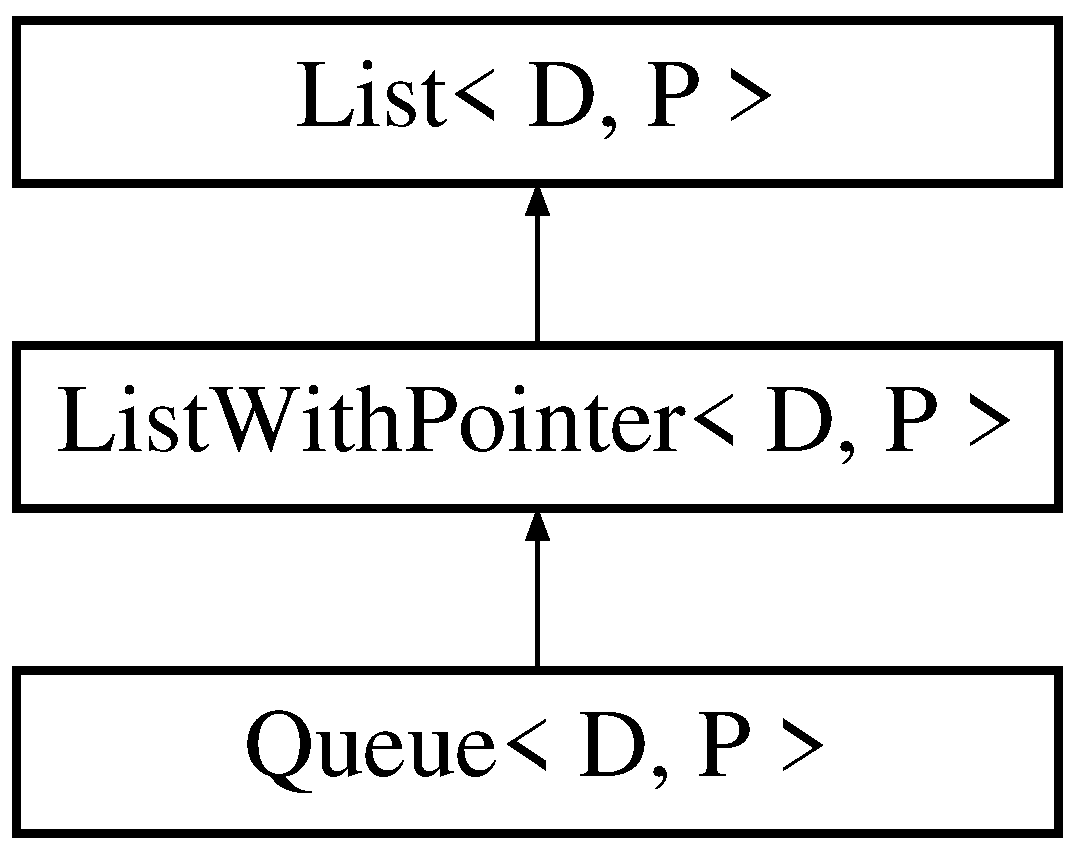
\includegraphics[height=3.000000cm]{class_queue}
\end{center}
\end{figure}
\subsection*{Public Member Functions}
\begin{DoxyCompactItemize}
\item 
\hyperlink{class_queue_aaecc8eba91905e5bda9752e0f85a150e}{Queue} ()
\begin{DoxyCompactList}\small\item\em Constructor de la clase \hyperlink{class_stack}{Stack}. \end{DoxyCompactList}\item 
\hyperlink{class_queue_a4934a19723695272d8722a8fc2d84240}{$\sim$\+Queue} ()
\begin{DoxyCompactList}\small\item\em Destructor de la clase \hyperlink{class_stack}{Stack}. \end{DoxyCompactList}\item 
void \hyperlink{class_queue_a896b0e1bcac0d660079eb838c1823446}{sort} ()
\begin{DoxyCompactList}\small\item\em Metodo que implementa el ordenar para \hyperlink{class_list_with_pointer}{List\+With\+Pointer}. \end{DoxyCompactList}\item 
void \hyperlink{class_queue_a8779ae337e779be3dbff7c7bb8285428}{push} (D d)
\begin{DoxyCompactList}\small\item\em Metodo que implementa el insertar (push) del \hyperlink{class_queue}{Queue}. \end{DoxyCompactList}\item 
void \hyperlink{class_queue_a1543a11927722a9ef59806e7119634c4}{pop} (D d)
\begin{DoxyCompactList}\small\item\em Metodo que implementa el sacar elemento del \hyperlink{class_queue}{Queue} (pop) \end{DoxyCompactList}\item 
P \hyperlink{class_queue_a5c5ad7000d15506d3ec9c2ef6c8e6041}{find} (D d)
\begin{DoxyCompactList}\small\item\em Metodo que implementa la busqueda en un \hyperlink{class_list_with_pointer}{List\+With\+Pointer}. \end{DoxyCompactList}\item 
int \hyperlink{class_queue_ab2c7217e6737bf579493b321184a2db3}{get\+Size} ()
\begin{DoxyCompactList}\small\item\em Metodo que implementa el obtener tamaño del \hyperlink{class_queue}{Queue}. \end{DoxyCompactList}\item 
void \hyperlink{class_queue_a5a68470adc616026ded26026bcec5a1f}{print\+Queue} ()
\begin{DoxyCompactList}\small\item\em Metodo para imprimir los elementos de la cola. \end{DoxyCompactList}\item 
P \hyperlink{class_queue_aa4c9b83f260a172e1fffc389f354386f}{next} (P k)
\begin{DoxyCompactList}\small\item\em Metodo que implementa el obtener siguiente elemento de una posicion especifica del \hyperlink{class_queue}{Queue}. \end{DoxyCompactList}\item 
P \hyperlink{class_queue_adcb9a0e709ea65bc7e98f7e9cbae8a39}{prev} (P k)
\begin{DoxyCompactList}\small\item\em Metodo que implementa el obtener elemento anterior en \hyperlink{class_queue}{Queue}. \end{DoxyCompactList}\item 
void \hyperlink{class_queue_a619e0caf9005be9ccd38e3284ad6b796}{empty\+Queue} ()
\begin{DoxyCompactList}\small\item\em Metodo que implementa el vaciar Cola que Deja sin ningun elemento el \hyperlink{class_queue}{Queue} e imprime cada elemento que retira. \end{DoxyCompactList}\end{DoxyCompactItemize}
\subsection*{Additional Inherited Members}


\subsection{Detailed Description}
\subsubsection*{template$<$typename D, typename P$>$class Queue$<$ D, P $>$}

Biblioteca que genera un template de la clase \hyperlink{class_stack}{Stack} (Pila) que hereda de la clase \hyperlink{class_list_with_pointer}{List\+With\+Pointer} y que toma un tipo de dato D para los datos contenidos con indices P. 

\subsection{Constructor \& Destructor Documentation}
\hypertarget{class_queue_aaecc8eba91905e5bda9752e0f85a150e}{\index{Queue@{Queue}!Queue@{Queue}}
\index{Queue@{Queue}!Queue@{Queue}}
\subsubsection[{Queue}]{\setlength{\rightskip}{0pt plus 5cm}template$<$typename D , typename P $>$ {\bf Queue}$<$ D, P $>$\+::{\bf Queue} (
\begin{DoxyParamCaption}
{}
\end{DoxyParamCaption}
)\hspace{0.3cm}{\ttfamily [inline]}}}\label{class_queue_aaecc8eba91905e5bda9752e0f85a150e}


Constructor de la clase \hyperlink{class_stack}{Stack}. 

\hypertarget{class_queue_a4934a19723695272d8722a8fc2d84240}{\index{Queue@{Queue}!````~Queue@{$\sim$\+Queue}}
\index{````~Queue@{$\sim$\+Queue}!Queue@{Queue}}
\subsubsection[{$\sim$\+Queue}]{\setlength{\rightskip}{0pt plus 5cm}template$<$typename D , typename P $>$ {\bf Queue}$<$ D, P $>$\+::$\sim${\bf Queue} (
\begin{DoxyParamCaption}
{}
\end{DoxyParamCaption}
)\hspace{0.3cm}{\ttfamily [inline]}}}\label{class_queue_a4934a19723695272d8722a8fc2d84240}


Destructor de la clase \hyperlink{class_stack}{Stack}. 



\subsection{Member Function Documentation}
\hypertarget{class_queue_a619e0caf9005be9ccd38e3284ad6b796}{\index{Queue@{Queue}!empty\+Queue@{empty\+Queue}}
\index{empty\+Queue@{empty\+Queue}!Queue@{Queue}}
\subsubsection[{empty\+Queue}]{\setlength{\rightskip}{0pt plus 5cm}template$<$typename D , typename P $>$ void {\bf Queue}$<$ D, P $>$\+::empty\+Queue (
\begin{DoxyParamCaption}
{}
\end{DoxyParamCaption}
)\hspace{0.3cm}{\ttfamily [inline]}}}\label{class_queue_a619e0caf9005be9ccd38e3284ad6b796}


Metodo que implementa el vaciar Cola que Deja sin ningun elemento el \hyperlink{class_queue}{Queue} e imprime cada elemento que retira. 

\hypertarget{class_queue_a5c5ad7000d15506d3ec9c2ef6c8e6041}{\index{Queue@{Queue}!find@{find}}
\index{find@{find}!Queue@{Queue}}
\subsubsection[{find}]{\setlength{\rightskip}{0pt plus 5cm}template$<$typename D , typename P $>$ P {\bf Queue}$<$ D, P $>$\+::find (
\begin{DoxyParamCaption}
\item[{D}]{d}
\end{DoxyParamCaption}
)\hspace{0.3cm}{\ttfamily [inline]}, {\ttfamily [virtual]}}}\label{class_queue_a5c5ad7000d15506d3ec9c2ef6c8e6041}


Metodo que implementa la busqueda en un \hyperlink{class_list_with_pointer}{List\+With\+Pointer}. 


\begin{DoxyParams}{Parameters}
{\em d} & Dato que se desea buscar en \hyperlink{class_list}{List} \\
\hline
\end{DoxyParams}
\begin{DoxyReturn}{Returns}
Indice de tipo P dentro de \hyperlink{class_list}{List} 
\end{DoxyReturn}


Reimplemented from \hyperlink{class_list_with_pointer_afeff8b963c197378553e2a3f73eaf66a}{List\+With\+Pointer$<$ D, P $>$}.

\hypertarget{class_queue_ab2c7217e6737bf579493b321184a2db3}{\index{Queue@{Queue}!get\+Size@{get\+Size}}
\index{get\+Size@{get\+Size}!Queue@{Queue}}
\subsubsection[{get\+Size}]{\setlength{\rightskip}{0pt plus 5cm}template$<$typename D , typename P $>$ int {\bf Queue}$<$ D, P $>$\+::get\+Size (
\begin{DoxyParamCaption}
{}
\end{DoxyParamCaption}
)\hspace{0.3cm}{\ttfamily [inline]}, {\ttfamily [virtual]}}}\label{class_queue_ab2c7217e6737bf579493b321184a2db3}


Metodo que implementa el obtener tamaño del \hyperlink{class_queue}{Queue}. 



Reimplemented from \hyperlink{class_list_with_pointer_ac70c49b5703887fd867e90cdac3c706f}{List\+With\+Pointer$<$ D, P $>$}.

\hypertarget{class_queue_aa4c9b83f260a172e1fffc389f354386f}{\index{Queue@{Queue}!next@{next}}
\index{next@{next}!Queue@{Queue}}
\subsubsection[{next}]{\setlength{\rightskip}{0pt plus 5cm}template$<$typename D , typename P $>$ P {\bf Queue}$<$ D, P $>$\+::next (
\begin{DoxyParamCaption}
\item[{P}]{k}
\end{DoxyParamCaption}
)\hspace{0.3cm}{\ttfamily [inline]}, {\ttfamily [virtual]}}}\label{class_queue_aa4c9b83f260a172e1fffc389f354386f}


Metodo que implementa el obtener siguiente elemento de una posicion especifica del \hyperlink{class_queue}{Queue}. 


\begin{DoxyParams}{Parameters}
{\em k} & Indice de tipo P dentro de \hyperlink{class_list}{List} del que se desea el siguiente elemento \\
\hline
\end{DoxyParams}
\begin{DoxyReturn}{Returns}
Siguiente elemento de k de tipo P 
\end{DoxyReturn}


Reimplemented from \hyperlink{class_list_with_pointer_a518b5ee89e3ad32ae7cd4ddd5d4fa7e9}{List\+With\+Pointer$<$ D, P $>$}.

\hypertarget{class_queue_a1543a11927722a9ef59806e7119634c4}{\index{Queue@{Queue}!pop@{pop}}
\index{pop@{pop}!Queue@{Queue}}
\subsubsection[{pop}]{\setlength{\rightskip}{0pt plus 5cm}template$<$typename D , typename P $>$ void {\bf Queue}$<$ D, P $>$\+::pop (
\begin{DoxyParamCaption}
\item[{D}]{d}
\end{DoxyParamCaption}
)\hspace{0.3cm}{\ttfamily [inline]}}}\label{class_queue_a1543a11927722a9ef59806e7119634c4}


Metodo que implementa el sacar elemento del \hyperlink{class_queue}{Queue} (pop) 

\begin{DoxyReturn}{Returns}
Puntero a la celda que contiene el dato sacado el \hyperlink{class_queue}{Queue} 
\end{DoxyReturn}
\hypertarget{class_queue_adcb9a0e709ea65bc7e98f7e9cbae8a39}{\index{Queue@{Queue}!prev@{prev}}
\index{prev@{prev}!Queue@{Queue}}
\subsubsection[{prev}]{\setlength{\rightskip}{0pt plus 5cm}template$<$typename D , typename P $>$ P {\bf Queue}$<$ D, P $>$\+::prev (
\begin{DoxyParamCaption}
\item[{P}]{k}
\end{DoxyParamCaption}
)\hspace{0.3cm}{\ttfamily [inline]}, {\ttfamily [virtual]}}}\label{class_queue_adcb9a0e709ea65bc7e98f7e9cbae8a39}


Metodo que implementa el obtener elemento anterior en \hyperlink{class_queue}{Queue}. 


\begin{DoxyParams}{Parameters}
{\em k} & Indice de tipo P dentro de la list del que se desea el elemento anterior \\
\hline
\end{DoxyParams}
\begin{DoxyReturn}{Returns}
Elemento anterior de k de tipo P 
\end{DoxyReturn}


Reimplemented from \hyperlink{class_list_with_pointer_a7242068fcc3a193f0f7e94517856e431}{List\+With\+Pointer$<$ D, P $>$}.

\hypertarget{class_queue_a5a68470adc616026ded26026bcec5a1f}{\index{Queue@{Queue}!print\+Queue@{print\+Queue}}
\index{print\+Queue@{print\+Queue}!Queue@{Queue}}
\subsubsection[{print\+Queue}]{\setlength{\rightskip}{0pt plus 5cm}template$<$typename D , typename P $>$ void {\bf Queue}$<$ D, P $>$\+::print\+Queue (
\begin{DoxyParamCaption}
{}
\end{DoxyParamCaption}
)\hspace{0.3cm}{\ttfamily [inline]}}}\label{class_queue_a5a68470adc616026ded26026bcec5a1f}


Metodo para imprimir los elementos de la cola. 

\hypertarget{class_queue_a8779ae337e779be3dbff7c7bb8285428}{\index{Queue@{Queue}!push@{push}}
\index{push@{push}!Queue@{Queue}}
\subsubsection[{push}]{\setlength{\rightskip}{0pt plus 5cm}template$<$typename D , typename P $>$ void {\bf Queue}$<$ D, P $>$\+::push (
\begin{DoxyParamCaption}
\item[{D}]{d}
\end{DoxyParamCaption}
)\hspace{0.3cm}{\ttfamily [inline]}}}\label{class_queue_a8779ae337e779be3dbff7c7bb8285428}


Metodo que implementa el insertar (push) del \hyperlink{class_queue}{Queue}. 


\begin{DoxyParams}{Parameters}
{\em d} & Elemento de tipo D que se inserta al \hyperlink{class_queue}{Queue} \\
\hline
\end{DoxyParams}
\hypertarget{class_queue_a896b0e1bcac0d660079eb838c1823446}{\index{Queue@{Queue}!sort@{sort}}
\index{sort@{sort}!Queue@{Queue}}
\subsubsection[{sort}]{\setlength{\rightskip}{0pt plus 5cm}template$<$typename D , typename P $>$ void {\bf Queue}$<$ D, P $>$\+::sort (
\begin{DoxyParamCaption}
{}
\end{DoxyParamCaption}
)\hspace{0.3cm}{\ttfamily [inline]}, {\ttfamily [virtual]}}}\label{class_queue_a896b0e1bcac0d660079eb838c1823446}


Metodo que implementa el ordenar para \hyperlink{class_list_with_pointer}{List\+With\+Pointer}. 

Implementacion por medio de Selection Sort

Implementacion por medio de Selection Sort 

Reimplemented from \hyperlink{class_list_with_pointer_aa46631b2da29895d1f767626fb591bc8}{List\+With\+Pointer$<$ D, P $>$}.



The documentation for this class was generated from the following file\+:\begin{DoxyCompactItemize}
\item 
include/\hyperlink{_queue_8h}{Queue.\+h}\end{DoxyCompactItemize}

\hypertarget{class_stack}{\section{Stack$<$ D, P $>$ Class Template Reference}
\label{class_stack}\index{Stack$<$ D, P $>$@{Stack$<$ D, P $>$}}
}


Libreria que genera un template de la clase \hyperlink{class_stack}{Stack} (Pila) que hereda de la clase \hyperlink{class_list_with_pointer}{List\+With\+Pointer} y que toma un tipo de dato D para los datos contenidos con indices P.  




{\ttfamily \#include $<$Stack.\+h$>$}

Inheritance diagram for Stack$<$ D, P $>$\+:\begin{figure}[H]
\begin{center}
\leavevmode
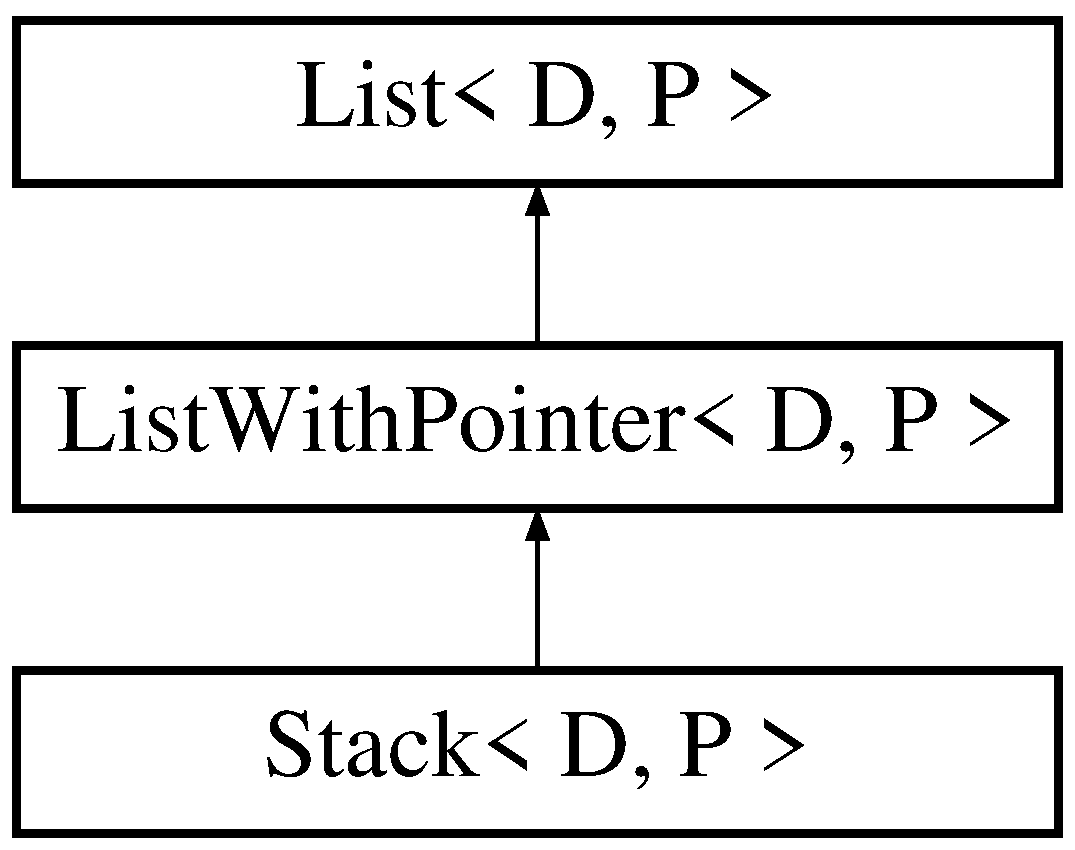
\includegraphics[height=3.000000cm]{class_stack}
\end{center}
\end{figure}
\subsection*{Public Member Functions}
\begin{DoxyCompactItemize}
\item 
\hyperlink{class_stack_a6e0f84830cde41cb8d49818842d18d36}{Stack} ()
\begin{DoxyCompactList}\small\item\em Constructor de la clase \hyperlink{class_stack}{Stack}. \end{DoxyCompactList}\item 
\hyperlink{class_stack_a181a491ce96ea87dc6db37e040f785e0}{$\sim$\+Stack} ()
\begin{DoxyCompactList}\small\item\em Destructor de la clase \hyperlink{class_stack}{Stack}. \end{DoxyCompactList}\item 
void \hyperlink{class_stack_ac023e5bfa5b4fc5a19d4a849fbfbbbcc}{push} (D d)
\begin{DoxyCompactList}\small\item\em Metodo que implementa el insertar (push) del \hyperlink{class_stack}{Stack}. \end{DoxyCompactList}\item 
\hyperlink{class_cell}{Cell}$<$ D $>$ $\ast$ \hyperlink{class_stack_ae874c09d418be57373d1a5bf5a6f27dd}{pop} ()
\begin{DoxyCompactList}\small\item\em Metodo que implementa el sacar elemento del S\+T\+A\+C\+K (pop) \end{DoxyCompactList}\item 
void \hyperlink{class_stack_ae8737ef6216bb3ee97e1cbf929395a9c}{top} ()
\begin{DoxyCompactList}\small\item\em Metodo que implementa el obtener el ultimo elemento del L\+I\+F\+O. \end{DoxyCompactList}\item 
void \hyperlink{class_stack_a045dffa682607b7eee938b900c5f698b}{empty\+Stack} ()
\begin{DoxyCompactList}\small\item\em Metodo que implementa el vaciar Pila que Deja sin ningun elemento el \hyperlink{class_stack}{Stack} e imprime cada elemento que retira. \end{DoxyCompactList}\item 
P \hyperlink{class_stack_aa8a3a0b773900e44f641e3be9d9345da}{find} (D d)
\begin{DoxyCompactList}\small\item\em Metodos que se heredan de \hyperlink{_list_with_pointer_8h}{List\+With\+Pointer.\+h}. \end{DoxyCompactList}\item 
P \hyperlink{class_stack_ab7f8f7e4ab10c00769c1debc5391fc17}{next} (P k)
\begin{DoxyCompactList}\small\item\em Metodo que implementa el obtener siguiente elemento de una posicion especifica del \hyperlink{class_stack}{Stack}. \end{DoxyCompactList}\item 
P \hyperlink{class_stack_a0c0b55f72c9249bfb9252bce1a93458d}{prev} (P k)
\begin{DoxyCompactList}\small\item\em Metodo que implementa el obtener elemento anterior en \hyperlink{class_stack}{Stack}. \end{DoxyCompactList}\item 
int \hyperlink{class_stack_a74fc7e5921dfb247f9ad7052c3c4297a}{get\+Size} ()
\begin{DoxyCompactList}\small\item\em Metodo que implementa el obtener tama�o del \hyperlink{class_stack}{Stack}. \end{DoxyCompactList}\end{DoxyCompactItemize}
\subsection*{Additional Inherited Members}


\subsection{Detailed Description}
\subsubsection*{template$<$typename D, typename P$>$class Stack$<$ D, P $>$}

Libreria que genera un template de la clase \hyperlink{class_stack}{Stack} (Pila) que hereda de la clase \hyperlink{class_list_with_pointer}{List\+With\+Pointer} y que toma un tipo de dato D para los datos contenidos con indices P. 

\subsection{Constructor \& Destructor Documentation}
\hypertarget{class_stack_a6e0f84830cde41cb8d49818842d18d36}{\index{Stack@{Stack}!Stack@{Stack}}
\index{Stack@{Stack}!Stack@{Stack}}
\subsubsection[{Stack}]{\setlength{\rightskip}{0pt plus 5cm}template$<$typename D , typename P $>$ {\bf Stack}$<$ D, P $>$\+::{\bf Stack} (
\begin{DoxyParamCaption}
{}
\end{DoxyParamCaption}
)\hspace{0.3cm}{\ttfamily [inline]}}}\label{class_stack_a6e0f84830cde41cb8d49818842d18d36}


Constructor de la clase \hyperlink{class_stack}{Stack}. 

\hypertarget{class_stack_a181a491ce96ea87dc6db37e040f785e0}{\index{Stack@{Stack}!````~Stack@{$\sim$\+Stack}}
\index{````~Stack@{$\sim$\+Stack}!Stack@{Stack}}
\subsubsection[{$\sim$\+Stack}]{\setlength{\rightskip}{0pt plus 5cm}template$<$typename D , typename P $>$ {\bf Stack}$<$ D, P $>$\+::$\sim${\bf Stack} (
\begin{DoxyParamCaption}
{}
\end{DoxyParamCaption}
)\hspace{0.3cm}{\ttfamily [inline]}}}\label{class_stack_a181a491ce96ea87dc6db37e040f785e0}


Destructor de la clase \hyperlink{class_stack}{Stack}. 



\subsection{Member Function Documentation}
\hypertarget{class_stack_a045dffa682607b7eee938b900c5f698b}{\index{Stack@{Stack}!empty\+Stack@{empty\+Stack}}
\index{empty\+Stack@{empty\+Stack}!Stack@{Stack}}
\subsubsection[{empty\+Stack}]{\setlength{\rightskip}{0pt plus 5cm}template$<$typename D , typename P $>$ void {\bf Stack}$<$ D, P $>$\+::empty\+Stack (
\begin{DoxyParamCaption}
{}
\end{DoxyParamCaption}
)\hspace{0.3cm}{\ttfamily [inline]}}}\label{class_stack_a045dffa682607b7eee938b900c5f698b}


Metodo que implementa el vaciar Pila que Deja sin ningun elemento el \hyperlink{class_stack}{Stack} e imprime cada elemento que retira. 

\hypertarget{class_stack_aa8a3a0b773900e44f641e3be9d9345da}{\index{Stack@{Stack}!find@{find}}
\index{find@{find}!Stack@{Stack}}
\subsubsection[{find}]{\setlength{\rightskip}{0pt plus 5cm}template$<$typename D , typename P $>$ P {\bf Stack}$<$ D, P $>$\+::find (
\begin{DoxyParamCaption}
\item[{D}]{d}
\end{DoxyParamCaption}
)\hspace{0.3cm}{\ttfamily [inline]}, {\ttfamily [virtual]}}}\label{class_stack_aa8a3a0b773900e44f641e3be9d9345da}


Metodos que se heredan de \hyperlink{_list_with_pointer_8h}{List\+With\+Pointer.\+h}. 

Metodo que implementa la busqueda en un \hyperlink{class_list_with_pointer}{List\+With\+Pointer} 
\begin{DoxyParams}{Parameters}
{\em d} & Dato que se desea buscar en \hyperlink{class_list}{List} \\
\hline
\end{DoxyParams}
\begin{DoxyReturn}{Returns}
Indice de tipo P dentro de \hyperlink{class_list}{List} 
\end{DoxyReturn}
Indicacion de que el dato no fue encontrado en la lista 

Reimplemented from \hyperlink{class_list_with_pointer_afeff8b963c197378553e2a3f73eaf66a}{List\+With\+Pointer$<$ D, P $>$}.

\hypertarget{class_stack_a74fc7e5921dfb247f9ad7052c3c4297a}{\index{Stack@{Stack}!get\+Size@{get\+Size}}
\index{get\+Size@{get\+Size}!Stack@{Stack}}
\subsubsection[{get\+Size}]{\setlength{\rightskip}{0pt plus 5cm}template$<$typename D , typename P $>$ int {\bf Stack}$<$ D, P $>$\+::get\+Size (
\begin{DoxyParamCaption}
{}
\end{DoxyParamCaption}
)\hspace{0.3cm}{\ttfamily [inline]}, {\ttfamily [virtual]}}}\label{class_stack_a74fc7e5921dfb247f9ad7052c3c4297a}


Metodo que implementa el obtener tama�o del \hyperlink{class_stack}{Stack}. 



Reimplemented from \hyperlink{class_list_with_pointer_ac70c49b5703887fd867e90cdac3c706f}{List\+With\+Pointer$<$ D, P $>$}.

\hypertarget{class_stack_ab7f8f7e4ab10c00769c1debc5391fc17}{\index{Stack@{Stack}!next@{next}}
\index{next@{next}!Stack@{Stack}}
\subsubsection[{next}]{\setlength{\rightskip}{0pt plus 5cm}template$<$typename D , typename P $>$ P {\bf Stack}$<$ D, P $>$\+::next (
\begin{DoxyParamCaption}
\item[{P}]{k}
\end{DoxyParamCaption}
)\hspace{0.3cm}{\ttfamily [inline]}, {\ttfamily [virtual]}}}\label{class_stack_ab7f8f7e4ab10c00769c1debc5391fc17}


Metodo que implementa el obtener siguiente elemento de una posicion especifica del \hyperlink{class_stack}{Stack}. 


\begin{DoxyParams}{Parameters}
{\em k} & Indice de tipo P dentro de \hyperlink{class_list}{List} del que se desea el siguiente elemento \\
\hline
\end{DoxyParams}
\begin{DoxyReturn}{Returns}
Siguiente elemento de k de tipo P 
\end{DoxyReturn}


Reimplemented from \hyperlink{class_list_with_pointer_a518b5ee89e3ad32ae7cd4ddd5d4fa7e9}{List\+With\+Pointer$<$ D, P $>$}.

\hypertarget{class_stack_ae874c09d418be57373d1a5bf5a6f27dd}{\index{Stack@{Stack}!pop@{pop}}
\index{pop@{pop}!Stack@{Stack}}
\subsubsection[{pop}]{\setlength{\rightskip}{0pt plus 5cm}template$<$typename D , typename P $>$ {\bf Cell}$<$D$>$$\ast$ {\bf Stack}$<$ D, P $>$\+::pop (
\begin{DoxyParamCaption}
{}
\end{DoxyParamCaption}
)\hspace{0.3cm}{\ttfamily [inline]}}}\label{class_stack_ae874c09d418be57373d1a5bf5a6f27dd}


Metodo que implementa el sacar elemento del S\+T\+A\+C\+K (pop) 

\begin{DoxyReturn}{Returns}
Puntero a la celda que contiene el dato sacado el S\+T\+A\+C\+K 
\end{DoxyReturn}
\hypertarget{class_stack_a0c0b55f72c9249bfb9252bce1a93458d}{\index{Stack@{Stack}!prev@{prev}}
\index{prev@{prev}!Stack@{Stack}}
\subsubsection[{prev}]{\setlength{\rightskip}{0pt plus 5cm}template$<$typename D , typename P $>$ P {\bf Stack}$<$ D, P $>$\+::prev (
\begin{DoxyParamCaption}
\item[{P}]{k}
\end{DoxyParamCaption}
)\hspace{0.3cm}{\ttfamily [inline]}, {\ttfamily [virtual]}}}\label{class_stack_a0c0b55f72c9249bfb9252bce1a93458d}


Metodo que implementa el obtener elemento anterior en \hyperlink{class_stack}{Stack}. 


\begin{DoxyParams}{Parameters}
{\em k} & Indice de tipo P dentro de la list del que se desea el elemento anterior \\
\hline
\end{DoxyParams}
\begin{DoxyReturn}{Returns}
Elemento anterior de k de tipo P 
\end{DoxyReturn}


Reimplemented from \hyperlink{class_list_with_pointer_a7242068fcc3a193f0f7e94517856e431}{List\+With\+Pointer$<$ D, P $>$}.

\hypertarget{class_stack_ac023e5bfa5b4fc5a19d4a849fbfbbbcc}{\index{Stack@{Stack}!push@{push}}
\index{push@{push}!Stack@{Stack}}
\subsubsection[{push}]{\setlength{\rightskip}{0pt plus 5cm}template$<$typename D , typename P $>$ void {\bf Stack}$<$ D, P $>$\+::push (
\begin{DoxyParamCaption}
\item[{D}]{d}
\end{DoxyParamCaption}
)\hspace{0.3cm}{\ttfamily [inline]}}}\label{class_stack_ac023e5bfa5b4fc5a19d4a849fbfbbbcc}


Metodo que implementa el insertar (push) del \hyperlink{class_stack}{Stack}. 


\begin{DoxyParams}{Parameters}
{\em d} & Elemento de tipo D que se inserta al S\+T\+A\+C\+K \\
\hline
\end{DoxyParams}
\hypertarget{class_stack_ae8737ef6216bb3ee97e1cbf929395a9c}{\index{Stack@{Stack}!top@{top}}
\index{top@{top}!Stack@{Stack}}
\subsubsection[{top}]{\setlength{\rightskip}{0pt plus 5cm}template$<$typename D , typename P $>$ void {\bf Stack}$<$ D, P $>$\+::top (
\begin{DoxyParamCaption}
{}
\end{DoxyParamCaption}
)\hspace{0.3cm}{\ttfamily [inline]}}}\label{class_stack_ae8737ef6216bb3ee97e1cbf929395a9c}


Metodo que implementa el obtener el ultimo elemento del L\+I\+F\+O. 

Imprime el ultimo elemento a�adido 

The documentation for this class was generated from the following file\+:\begin{DoxyCompactItemize}
\item 
include/\hyperlink{_stack_8h}{Stack.\+h}\end{DoxyCompactItemize}

\chapter{File Documentation}
\hypertarget{_cell_8h}{\section{include/gwp/\+Cell.h File Reference}
\label{_cell_8h}\index{include/gwp/\+Cell.\+h@{include/gwp/\+Cell.\+h}}
}
{\ttfamily \#include $<$iostream$>$}\\*
Include dependency graph for Cell.\+h\+:
This graph shows which files directly or indirectly include this file\+:
\subsection*{Classes}
\begin{DoxyCompactItemize}
\item 
class \hyperlink{class_cell}{Cell$<$ D $>$}
\begin{DoxyCompactList}\small\item\em Libreria que genera un template de una clase \hyperlink{class_cell}{Cell} que contiene datos de tipo D. \end{DoxyCompactList}\end{DoxyCompactItemize}

\hypertarget{_list_8h}{\section{include/\+List.h File Reference}
\label{_list_8h}\index{include/\+List.\+h@{include/\+List.\+h}}
}
This graph shows which files directly or indirectly include this file\+:
\subsection*{Classes}
\begin{DoxyCompactItemize}
\item 
class \hyperlink{class_list}{List$<$ D, P $>$}
\begin{DoxyCompactList}\small\item\em Libreria que genera un template de una clase abstracta list. \end{DoxyCompactList}\end{DoxyCompactItemize}

\hypertarget{_list_with_array_8h}{\section{include/\+List\+With\+Array.h File Reference}
\label{_list_with_array_8h}\index{include/\+List\+With\+Array.\+h@{include/\+List\+With\+Array.\+h}}
}
{\ttfamily \#include $<$iostream$>$}\\*
{\ttfamily \#include \char`\"{}List.\+h\char`\"{}}\\*
Include dependency graph for List\+With\+Array.\+h\+:
This graph shows which files directly or indirectly include this file\+:
\subsection*{Classes}
\begin{DoxyCompactItemize}
\item 
class \hyperlink{class_list_with_array}{List\+With\+Array$<$ D, P $>$}
\begin{DoxyCompactList}\small\item\em Libreria que genera un template de una clase \hyperlink{class_list_with_array}{List\+With\+Array} (lista implementada con arreglos) que hereda de la clase \hyperlink{class_list}{List} y que toma un tipo de dato para los datos contenidos en la lista (D) y otro para los indices de las misma (P) \end{DoxyCompactList}\end{DoxyCompactItemize}

\hypertarget{_list_with_pointer_8h}{\section{include/gwp/\+List\+With\+Pointer.h File Reference}
\label{_list_with_pointer_8h}\index{include/gwp/\+List\+With\+Pointer.\+h@{include/gwp/\+List\+With\+Pointer.\+h}}
}
{\ttfamily \#include $<$iostream$>$}\\*
{\ttfamily \#include \char`\"{}List.\+h\char`\"{}}\\*
{\ttfamily \#include \char`\"{}Cell.\+h\char`\"{}}\\*
Include dependency graph for List\+With\+Pointer.\+h\+:
This graph shows which files directly or indirectly include this file\+:
\subsection*{Classes}
\begin{DoxyCompactItemize}
\item 
class \hyperlink{class_list_with_pointer}{List\+With\+Pointer$<$ D, P $>$}
\begin{DoxyCompactList}\small\item\em Libreria que genera un template de una clase \hyperlink{class_list_with_pointer}{List\+With\+Pointer} (lista implementada con punteros) que hereda de la clase \hyperlink{class_list}{List} y que toma un tipo de dato para los datos contenidos en la lista (D) y otro para los indices de las misma (P) \end{DoxyCompactList}\end{DoxyCompactItemize}

\hypertarget{_queue_8h}{\section{include/\+Queue.h File Reference}
\label{_queue_8h}\index{include/\+Queue.\+h@{include/\+Queue.\+h}}
}
{\ttfamily \#include $<$iostream$>$}\\*
{\ttfamily \#include \char`\"{}List\+With\+Pointer.\+h\char`\"{}}\\*
{\ttfamily \#include \char`\"{}Cell.\+h\char`\"{}}\\*
\subsection*{Classes}
\begin{DoxyCompactItemize}
\item 
class \hyperlink{class_queue}{Queue$<$ D, P $>$}
\begin{DoxyCompactList}\small\item\em Biblioteca que genera un template de la clase \hyperlink{class_stack}{Stack} (Pila) que hereda de la clase \hyperlink{class_list_with_pointer}{List\+With\+Pointer} y que toma un tipo de dato D para los datos contenidos con indices P. \end{DoxyCompactList}\end{DoxyCompactItemize}

\hypertarget{_stack_8h}{\section{include/\+Stack.h File Reference}
\label{_stack_8h}\index{include/\+Stack.\+h@{include/\+Stack.\+h}}
}
{\ttfamily \#include $<$iostream$>$}\\*
{\ttfamily \#include \char`\"{}List\+With\+Pointer.\+h\char`\"{}}\\*
{\ttfamily \#include \char`\"{}Cell.\+h\char`\"{}}\\*
\subsection*{Classes}
\begin{DoxyCompactItemize}
\item 
class \hyperlink{class_stack}{Stack$<$ D, P $>$}
\begin{DoxyCompactList}\small\item\em Libreria que genera un template de la clase \hyperlink{class_stack}{Stack} (Pila) que hereda de la clase \hyperlink{class_list_with_pointer}{List\+With\+Pointer} y que toma un tipo de dato D para los datos contenidos con indices P. \end{DoxyCompactList}\end{DoxyCompactItemize}

\hypertarget{main_8cpp}{\section{src/main.cpp File Reference}
\label{main_8cpp}\index{src/main.\+cpp@{src/main.\+cpp}}
}
{\ttfamily \#include \char`\"{}../include/\+D\+N\+Acompare.\+h\char`\"{}}\\*
Include dependency graph for main.\+cpp\+:
\subsection*{Macros}
\begin{DoxyCompactItemize}
\item 
\#define \hyperlink{main_8cpp_af316c33cc298530f245e8b55330e86b5}{D}~int
\begin{DoxyCompactList}\small\item\em Universidad de Costa Rica -\/ Escuela de Ingenieria E\+Lectrica I\+E-\/0217 -\/ P\+R\+O\+Y\+E\+C\+T\+O\+: Comparacion de secuencias de nucleotidos de A\+D\+N utilizando el algoritmo Aho-\/\+Corasick. \end{DoxyCompactList}\end{DoxyCompactItemize}
\subsection*{Functions}
\begin{DoxyCompactItemize}
\item 
int \hyperlink{main_8cpp_a3c04138a5bfe5d72780bb7e82a18e627}{main} (int argc, char $\ast$$\ast$argv)
\begin{DoxyCompactList}\small\item\em Main del programa que realiza las pruebas del Algoritmo Aho-\/\+Corasick implementado en comparacion de cadenas de nucleotidos de A\+D\+N. \end{DoxyCompactList}\end{DoxyCompactItemize}


\subsection{Macro Definition Documentation}
\hypertarget{main_8cpp_af316c33cc298530f245e8b55330e86b5}{\index{main.\+cpp@{main.\+cpp}!D@{D}}
\index{D@{D}!main.\+cpp@{main.\+cpp}}
\subsubsection[{D}]{\setlength{\rightskip}{0pt plus 5cm}\#define D~int}}\label{main_8cpp_af316c33cc298530f245e8b55330e86b5}


Universidad de Costa Rica -\/ Escuela de Ingenieria E\+Lectrica I\+E-\/0217 -\/ P\+R\+O\+Y\+E\+C\+T\+O\+: Comparacion de secuencias de nucleotidos de A\+D\+N utilizando el algoritmo Aho-\/\+Corasick. 

\begin{DoxyAuthor}{Author}
Luis Adrian Aguilar Cascante -\/ B00092 

Robin Gonzalez -\/ B43011 

Giancarlo Marin -\/ B54099 
\end{DoxyAuthor}
\begin{DoxyDate}{Date}
26-\/02-\/2017 Programa de prueba para el funcionamiento de la comparacion de nucleotidos 
\end{DoxyDate}


Definition at line 11 of file main.\+cpp.



\subsection{Function Documentation}
\hypertarget{main_8cpp_a3c04138a5bfe5d72780bb7e82a18e627}{\index{main.\+cpp@{main.\+cpp}!main@{main}}
\index{main@{main}!main.\+cpp@{main.\+cpp}}
\subsubsection[{main}]{\setlength{\rightskip}{0pt plus 5cm}int main (
\begin{DoxyParamCaption}
\item[{int}]{argc, }
\item[{char $\ast$$\ast$}]{argv}
\end{DoxyParamCaption}
)}}\label{main_8cpp_a3c04138a5bfe5d72780bb7e82a18e627}


Main del programa que realiza las pruebas del Algoritmo Aho-\/\+Corasick implementado en comparacion de cadenas de nucleotidos de A\+D\+N. 


\begin{DoxyParams}{Parameters}
{\em int} & Indicador de la cantidad de argumentos pasados en la ejecucion del programa \\
\hline
{\em char$\ast$$\ast$} & Vector de char$\ast$ que contiene los argumentos enviados al ejecutar el programa \\
\hline
\end{DoxyParams}
\begin{DoxyReturn}{Returns}

\end{DoxyReturn}


Definition at line 21 of file main.\+cpp.


%--- End generated contents ---

% Index
\newpage
\phantomsection
\addcontentsline{toc}{chapter}{Index}
\printindex

\end{document}
